\documentclass[a4paper,12pt]{extbook} % Loads settings for the document layout



\usepackage{statecharts-style}

% % % % % % % % % % % % % % % % % % % %
% COOPERATION

\newcommand{\DoneByGA}[1]{\textcolor{OliveGreen}{ #1}}
\newcommand{\GAcomment}[1]{{\DoneByGA{GIORGIO SAYS:#1}}}
\newcommand{\GAmarg}[1]{\todo{\textcolor{green}{#1}}}

\newcommand{\DoneByFD}[1]{\textcolor{magenta}{#1}}
\newcommand{\FDcomment}[1]{{\DoneByFD{FERRUCCIO SAYS:#1}}}
\newcommand{\FDmarg}[1]{\todo{\textcolor{magenta}{#1}}}
\newcommand{\FDdel}[1]{\textcolor{magenta}{\sout{#1}}}
\newcommand{\FDadd}[1]{{\color{magenta}{#1}}}

\newcommand{\DoneByMV}[1]{\textcolor{blue}{ #1}}
\newcommand{\MVcomment}[1]{{\DoneByMV{MIRKO SAYS:#1}}}
\newcommand{\MVmarg}[1]{\todo{\textcolor{blue}{#1}}}
\newcommand{\MVdel}[1]{\textcolor{blue}{\sout{#1}}}
\newcommand{\MVadd}[1]{{\textcolor{blue}{#1}}}

\newcommand{\JBmarg}[1]{\todo{\textcolor{red}{#1}}}
\newcommand{\JBdel}[1]{\textcolor{red}{\sout{#1}}}
\newcommand{\JBadd}[1]{{\textcolor{red}{#1}}}

\newcommand{\FORGET}[1]{}
\newcommand{\HFCprime}{$\text{HFC}'$}
\newcommand{\coherentEnv}[3]{\textit{WFVTE}(#3;#1)}


% % % % % % % % % % % % % % % % % % % %
% CALCULUS

\newcommand{\trans}[2]{\mathcal{T}_{#1} \llbracket #2 \rrbracket}

\newcommand{\HFC}{HFC}
\newcommand{\FSCAFI}{{\sc{}FScaFi}\xspace}
\newcommand{\FSCAFIi}{{\sc{}FScaFi$'$}\xspace}
\newcommand{\FeatherweightSCAFI}{{\sc{}Featherweight ScaFi}\xspace}

\newcommand{\BNFcce}{{ ::=}}
\newcommand{\BNFmid}{\;\bigr\rvert\;}

\newcommand{\PROGRAM}{\mathtt{P}}
\newcommand{\FUNCTION}{\mathtt{F}}
\newcommand{\IMPORT}{\mathtt{I}}

\newcommand{\main}{\mathtt{main}}
\newcommand{\e}{\mathtt{e}}
\newcommand{\s}{\mathtt{s}}
\newcommand{\emain}{\e_{\main}}
\newcommand{\fname}{\mathtt{d}}
\newcommand{\xname}{\mathtt{x}}
\newcommand{\yname}{\mathtt{y}}
\newcommand{\zname}{\mathtt{z}}
\newcommand{\bname}{\mathtt{b}}
\newcommand{\oname}{\mathtt{o}}
\newcommand{\ofname}{\mathtt{g}}
\newcommand{\iname}{\mathtt{m}}

\newcommand{\lvalueSet}{\mathcal{L}}

\newcommand{\anyvalue}{\mathtt{v}}
\newcommand{\lvalue}{\ell}
\newcommand{\fvalue}{\phi}
\newcommand{\funvalue}{\mathtt{f}}
\newcommand{\svalue}{\mathtt{s}}
\newcommand{\snvalue}{\mathtt{r}}
\newcommand{\truevalue}{\mathtt{True}}
\newcommand{\falsevalue}{\mathtt{False}}
\newcommand{\zerovalue}{0}

\newcommand{\dc}{\mathtt{c}}
\newcommand{\dcOf}[2]{#1(#2)}

\newcommand{\auxNAME}{\textit{aux}}
\newcommand{\aux}[1]{\auxNAME(#1)}
\newcommand{\bodyNAME}{\textit{
body}}
\newcommand{\body}[1]{\bodyNAME(#1)}
\newcommand{\argsNAME}{\textit{args}}
\newcommand{\args}[1]{\argsNAME(#1)}
\newcommand{\nameOf}{\textit{name}}

\newcommand{\FVname}{\textbf{FV}}
\newcommand{\FV}[1]{\FVname(#1)}
\newcommand{\FTVname}{\textbf{FTV}}
\newcommand{\FTV}[1]{\FTVname(#1)}

\newcommand{\spawnK}{\mathtt{spawn}}
\newcommand{\defK}{\mathtt{def}}
\newcommand{\nbrK}{\mathtt{nbr}}
\newcommand{\repK}{\mathtt{rep}}
\newcommand{\shareK}{\mathtt{share}}
\newcommand{\fifK}{\mathtt{if}}
\newcommand{\elseK}{\mathtt{else}}
\newcommand{\ifK}{\mathtt{branch}}
\newcommand{\foldK}{\mathtt{foldhood}}
\newcommand{\foldexclK}{\mathtt{foldhoodPlus}}
\newcommand{\foldincK}{\mathtt{foldincl}}
\newcommand{\letK}{\mathtt{let}\;}
\newcommand{\inK}{\;\mathtt{in}\;}

\newcommand{\aggrK}{@@}
\newcommand{\eqSymK}[1]{\mathrm{ \texttt{= \aggrK \{} #1 \texttt{\}} }}
\newcommand{\ftoSymK}[1]{\mathrm{ \texttt{=>\{}#1\texttt{\}} }}
\newcommand{\ftoSym}[1]{\mathrm{ \texttt{=>}#1 }}
\newcommand{\toSymK}[1]{\mathrm{ \texttt{=> \aggrK\{} #1 \texttt{\}} }}
\newcommand{\toSymKtag}[2]{\toSym{#1}\mathrm{ \texttt{\aggrK\{} #2 \texttt{\}}}}
\newcommand{\toSymKabs}[1]{\mathrm{ \texttt{=>} #1  }}

\newcommand{\toSym}[1]{\stackrel{#1}{\mathrm{\texttt{=>}}}}
\renewcommand{\name}{\tau}


\newcommand{\fstK}{\mathtt{fst}}
\newcommand{\sndK}{\mathtt{snd}}
\newcommand{\headK}{\mathtt{head}}
\newcommand{\tailK}{\mathtt{tail}}

\newcommand{\setK}{\mathtt{set}}
\newcommand{\mapK}{\mathtt{map}}
\newcommand{\pairK}{\mathtt{pair}}
\newcommand{\consK}{\mathtt{cons}}
\newcommand{\PairK}{\mathtt{Pair}}
\newcommand{\NullK}{\mathtt{Null}}
\newcommand{\ConsK}{\mathtt{Cons}}
\newcommand{\listK}{\mathtt{list}}

\newcommand{\pairltypeOf}[2]{\pairK(#1,#2)}
\newcommand{\listltypeOf}[1]{\listK(#1)}

\newcommand{\nbrlt}{\mathtt{nbrlt}}

\newcommand{\selfK}{\mathtt{uid}}
\newcommand{\muxK}{\mathtt{mux}}
\newcommand{\minHoodK}{\texttt{minhood}}
\newcommand{\pickHoodK}{\texttt{pickhood}}
\newcommand{\snsNumK}{\texttt{snsnum}}
\newcommand{\snsFunK}{\texttt{snsfun}}


% % % % % % % % % % % % % % % % % % % %
% TYPING

\newcommand{\type}{\textit{T}}
\newcommand{\ltype}{\textit{L}}
\newcommand{\ftype}{\textit{F}}
\newcommand{\rtype}{\textit{R}}
\newcommand{\stype}{\textit{S}}
\newcommand{\builtintype}{\textit{B}}

\newcommand{\ftypeOf}[1]{\mathtt{field}(#1)}

\newcommand{\btype}{\mathtt{bool}}
\newcommand{\ntype}{\mathtt{num}}

\newcommand{\stvar}{s}
\newcommand{\rtvar}{r}
\newcommand{\ltvar}{l}
\newcommand{\tvar}{t}

\newcommand{\typescheme}{\textit{TS}}
\newcommand{\ltypescheme}{\textit{LS}}

\newcommand{\TtypEnv}{\mathcal{A}}
\newcommand{\OStypEnv}{\mathcal{B}}
\newcommand{\TStypEnv}{\mathcal{D}}
\newcommand{\LTStypEnv}{\mathcal{D}}
\newcommand{\typeofNAME}{\OStypEnv}
\newcommand{\typeof}[1]{\typeofNAME(#1)}

\newcommand{\expTypJud}[4]{#1 ; #2 \vdash #3 : #4}
\newcommand{\funTypJud}[3]{#1 \vdash #2 : #3}
\newcommand{\proTypJud}[2]{\vdash #1 : #2}

\newcommand{\surfaceTyping}[3]{
  \begin{array}{l@{\;}c}
    \stackrel{~}{{\tiny \textrm{[#1]}}} & #2 \\ \hline 
    \multicolumn{2}{c}{#3}
  \end{array}
}
\newcommand{\nullsurfaceTyping}[2]{
  \surfaceTyping{#1}{}{#2}
}


% % % % % % % % % % % % % % % % % % % %
% OPERATIONAL SEMANTICS

\newcommand{\deviceIdSet}{\textbf{D}}
\newcommand{\builtinop}[3]{\llparenthesis #1 \rrparenthesis_{#2}^{#3}}
\newcommand{\filter}{F}

\newcommand{\Trees}{\Theta}
\renewcommand{\emptyseq}{\bullet}

\newcommand{\devset}{I}
\newcommand{\Topo}{\tau}
\newcommand{\Sens}{\Sigma}
\newcommand{\Envi}{\textit{Env}}
\newcommand{\EnviS}[2]{#1,#2}
\newcommand{\SystS}[2]{\langle #1;#2\rangle}
\newcommand{\Field}{\Psi}
\newcommand{\Cfg}{N}
\newcommand{\wfn}[1]{\textit{WFE}(#1)}
\newcommand{\senstate}{\sigma}

\newcommand{\nettran}[3]{#1\xrightarrow{#2} #3}
\newcommand{\act}{\textit{act}}
\newcommand{\envact}{\textit{env}}

\newcommand{\envmap}[2]{#1\mapsto #2}
\newcommand{\mapupdate}[2]{#1[#2]}
\newcommand{\proj}[2]{{#1}|_{#2}}

\newcommand{\ruleNameSize}[1]{{\scriptsize #1}}

\newcommand{\domofNAME}{\mathcal{D}}
\newcommand{\domof}[1]{\domofNAME_{#1}}
\newcommand{\erasureofNAME}{\textbf{erasure}}
\newcommand{\erasureof}[1]{\erasureofNAME(#1)}

\newcommand{\vtree}{\theta}
\newcommand{\mkvtree}[3]{#2 \langle #3 \rangle}
\newcommand{\mkvt}[2]{#1 \langle #2 \rangle}
\newcommand{\piB}[1]{\pi^{#1}}
\newcommand{\piBof}[2]{\piB{#1}(#2)}
\newcommand{\piI}[1]{\pi_{#1}}
\newcommand{\piIof}[2]{\piI{#1}(#2)}
\newcommand{\piIofOv}[1]{\overline{\pi}(#1)}

\newcommand{\lengthOf}[1]{\textit{length}(#1)}

\newcommand{\bsopsem}[5]{#1;#2;#3\vdash #4\Downarrow #5}
\newcommand{\deviceId}{\delta}
\newcommand{\vroot}{\mathbf{\rho}}
\newcommand{\vrootOf}[1]{\vroot(#1)}
\newcommand{\substitution}[2]{#1:=#2}
\newcommand{\applySubstitution}[2]{#1[#2]}
\newcommand{\bsopsemFAIL}[4]{#1;#2;#3\vdash #4\;\FAIL}
\newcommand{\FAIL}{\textup{\textsc{fail}}}


\newcommand{\skiptransition}{\\[10pt]}
\newcommand{\skiptransitionR}{\\[-3pt]}
\newcommand{\skiptransitionN}{\\[-2.22pt]}

\newcommand{\netopsemRule}[3]{\surfaceTyping{#1}{#2}{#3}}

\newcommand{\coherent}[3]{\mathcal{C}^{#2}_{#3}[#1]}

%\newcommand{\denotf}[2]{\lambda #1.#2}


% % % % % % % % % % % % % % % % % % % %
% DENOTATIONAL SEMANTICS
\DeclareMathOperator{\lightcone}{LC}
\DeclareMathOperator{\connected}{CD}
\newcommand{\disjcup}{\biguplus}
\newcommand{\powerset}{\mathcal{P}}
\newcommand{\shift}[1]{\textbf{shift}(#1)}
\newcommand{\builtindenot}[2]{\mathcal{#1}\llbracket #2 \rrbracket}
\newcommand{\predevices}[1]{{#1}^{{}^-}\!\!\!}
\newcommand{\nbrdevice}[2]{{#1}^{#2}}
\newcommand{\repdevice}[1]{{#1}^-}
\newcommand{\decay}[0]{t_{\mathtt{d}}}
\newcommand{\FieldS}[0]{\mathcal{F}}
\newcommand{\PathS}[0]{\mathbf{P}}
\newcommand{\pathS}[0]{P}
\newcommand{\VarS}[0]{X}
\newcommand{\varS}[0]{\mathtt{X}}
\DeclareMathOperator{\rank}{rank}
\newcommand{\aEventS}[0]{\mathbb{E}}
\newcommand{\EventCone}[0]{\mathbf{EC}}
\newcommand{\EventSet}[0]{\mathbf{ES}}
\newcommand{\EventS}[0]{\mathbf{E}}
\newcommand{\eventS}[0]{E}
\newcommand{\eventId}[0]{\epsilon}
\newcommand{\timeS}[0]{t}
\newcommand{\posS}[0]{p}
\newcommand{\event}[3]{\langle #1,#2,#3\rangle}
\newcommand{\devF}[1]{\deviceId_{#1}}
\newcommand{\timeF}[1]{\timeS_{#1}}
\newcommand{\posF}[1]{\posS_{#1}}
\newcommand{\domS}[0]{D}
\newcommand{\DomS}[0]{\mathcal{D}}
\newcommand{\DomDevF}[2]{#1(#2)}
\newcommand{\DomTimeF}[2]{#1(#2)}
\newcommand{\DomMTimeF}[2]{#1^{-}(#2)}
\newcommand{\DomDomF}[2]{#1(#2)}
\newcommand{\DomDevTimeF}[3]{#1(#2,#3)}
\newcommand{\DomDevMTimeF}[3]{#1^{-}(#2,#3)}

\newcommand{\feS}[0]{\Phi}
\newcommand{\setVS}[0]{\textbf{V}}
\newcommand{\setTS}[0]{\textbf{T}}
\newcommand{\setCS}[0]{\textbf{C}}
\newcommand{\setFS}[0]{\textbf{F}}

\newcommand{\pto}{\mathrel{\ooalign{\hfil$\mapstochar$\hfil\cr$\to$\cr}}}
\newcommand{\neighbour}[2]{\textit{neigh}(#1,#2)}
\newcommand{\neigh}{\rightsquigarrow}

\newcommand{\denot}[1]{\mathcal{E}\llbracket{#1}\rrbracket}
\newcommand{\denotapp}[2]{\denot{#1}_{#2}}
\newcommand{\denotappsub}[3]{\denot{#1}_{#2}^{#3}}
\newcommand{\denotfun}[3]{\mathcal{L}\llbracket{#1}\rrbracket_{#2}^{#3}}
\newcommand{\denottype}[1]{\mathcal{T}\llbracket{#1}\rrbracket}
\newcommand{\denotval}[1]{\mathcal{V}\llbracket {#1} \rrbracket}
\newcommand{\denotexp}[3]{\mathcal{E}\llbracket {#1} \rrbracket_{#2}^{#3}}
\newcommand{\denotf}[2]{\lambda #1.#2}
\newcommand{\dvalue}[0]{\mathrm{\Phi}}


% % % % % % % % % % % % % % % % % % % %
% CODE HIGHLIGHTING

\definecolor{dark-gray}{gray}{0}
\newcommand{\il}[1]{{\it \textcolor{dark-gray}{// #1}}} % inline comment
\newcommand{\km}[1]{{\textcolor{red}{#1}}} % key mechanism primitives
\renewcommand{\fn}[1]{\textcolor{violet}{#1}} % function calls
\newcommand{\pr}[1]{\texttt{\textcolor{blue}{#1}}} % primitives
\newcommand{\high}[1]{\underline{#1}} % highlight currently executed subexpression


% % % % % % % % % % % % % % % % % % % %
% PARENTHESIS

\newcommand{\cp}[1]{\left( #1 \right)}
\newcommand{\qp}[1]{\left[ #1 \right]}
%\newcommand{\Qp}[1]{\left\llbracket #1 \right\rrbracket}
%\newcommand{\ap}[1]{\left\langle #1 \right\rangle}
\newcommand{\ap}[1]{\langle #1 \rangle}
\newcommand{\bp}[1]{\left\lbrace #1 \right\rbrace}
\newcommand{\vp}[1]{\left\lvert #1 \right\rvert}
\newcommand{\floor}[1]{\left\lfloor #1 \right\rfloor}
\newcommand{\ceil}[1]{\left\lceil #1 \right\rceil}


% % % % % % % % % % % % % % % % % % % %
% MISC

\DeclareMathOperator{\norm}{norm}
\DeclareMathOperator{\dist}{dist}

\newcommand{\res}{\upharpoonright}

\newcommand{\stval}[1]{\setVS(#1)}
\newcommand{\stvals}{\stval{\ast}}
\newcommand{\stvalc}{\stval{\top}}

\newcommand{\TMc}{\text{TM}_{\textit{cone}}}
\newcommand{\TMl}{\text{TM}_{\textit{loc}}}

\newcommand{\restatement}[4]{\noindent \textbf{Restatement of #1 \ref{#2} (#3).} \textit{#4}}

\newcommand{\ifKhfc}{\mathtt{if}}

\newcommand{\corrstart}{}%{\color{magenta}}
\newcommand{\corrend}{}%{\color{black}}
\newcommand{\correction}[1]{\corrstart #1\corrend{}}

\newcommand{\corrstartB}{\color{magenta}}
\newcommand{\correndB}{\color{black}}
\newcommand{\correctionB}[1]{\corrstartB #1\correndB{}}



\definecolor{mygreen}{rgb}{0,0.6,0}
\definecolor{mygray}{rgb}{0.5,0.5,0.5}
\definecolor{mymauve}{rgb}{0.58,0,0.82}
\definecolor{darkgreen}{rgb}{0,0.5,0}
\definecolor{mylightgray}{rgb}{0.97,0.97,0.97}

\lstdefinelanguage{Protelis}{
    language=Java,
    morecomment=[l]{//},
    morecomment=[s]{/*}{*/},
    keywords={def, else, import, mux, sumHood, PlusSelf, let, rep, env, self, pi, if, e, public, NaN, false, true, minHood, maxHood, nbrRange, nbr, Infinity},
    frame=no,
    breaklines=true,
    captionpos=b,
    keepspaces=true,
    backgroundcolor=\color{mylightgray},    
    basicstyle=\ttfamily\small,
    keywordstyle=\bfseries\color{red},
    emphstyle={\bfseries\color{blue}},
    stringstyle=\ttfamily\color{purple},
    commentstyle=\ttfamily\color{mygreen}
}

\lstdefinelanguage{scafi}{
  keywords={abstract,case,catch,class,def,%
    do,else,extends,final,finally,%
    for,if,implicit,import,match,mixin,%
    new,null,object,override,package,%
    private,protected,requires,return,sealed,%
    super,this,throw,trait,try,lazy,%
    type,val,var,while,with,yield,forSome},
  otherkeywords={=>,<-,<\%,<:,>:,\#},
  keywordstyle=\color{blue},
  keywordstyle=[2]\color{red}\textbf,
  keywords=[2]{rep,nbr,foldhood,@@},
  keywordstyle=[3]\color{violet}\textbf,
  keywords=[3]{nbrvar,sense,branch,mid,mux,nbrRange,sumHood,pickHood,
  	countHood,minHood,maxHood,foldhoodPlus,G,C,S,T,broadcast,
  	distanceTo,summarize,minHoodPlus,gradient,
  	collectSets,collectSet,priorityS,Metric},
  keywordstyle=[4]\color{orange},
  keywordstyle=[5]\color{darkgray},
  sensitive=true,
  morecomment=[l]{//},
  morecomment=[n]{/*}{*/},
  commentstyle=\color{mygreen},
  morestring=[b]",
  morestring=[b]',
  morestring=[b]""",
  moredelim=[is][\color{gray}\bfseries\underbar]{?-}{-?}
} 

\lstdefinelanguage{fscafi}{
  keywords={abstract,case,catch,class,def,%
    do,else,extends,final,finally,%
    for,if,implicit,import,match,mixin,%
    new,null,object,override,package,%
    private,protected,requires,return,sealed,%
    super,this,throw,trait,try,lazy,%
    type,val,var,while,with,yield,forSome},
  otherkeywords={=>,<-,<\%,<:,>:,\#},
  keywordstyle=\color{black}\textbf,
  keywordstyle=[2]\color{black}\textbf,
  keywords=[2]{rep,nbr,foldhood,branch,@@},
  keywordstyle=[3]\color{black}\textbf,
  keywords=[3]{false,true,nbrvar,sense,mid,mux,nbrRange,sumHood,pickHood,countHood,minHood,maxHood,foldhoodPlus,G,C,S,T,broadcast,distanceTo,summarize,minHoodPlus},
  keywordstyle=[4]\color{black},
  keywordstyle=[5]\color{black},
  sensitive=true,
  morecomment=[l]{//},
  morecomment=[n]{/*}{*/},
  commentstyle=\color{darkgreen},
  morestring=[b]",
  morestring=[b]',
  morestring=[b]""",
  basicstyle=\lst@ifdisplaystyle\small\fi\ttfamily
} 

\lstdefinestyle{mystyle}{showstringspaces=false,keepspaces=true,basicstyle=\small\lst@ifdisplaystyle\footnotesize\selectfont\fi\ttfamily,commentstyle=\itshape,stringstyle=\sffamily,backgroundcolor = \color{lightgray!8},frame=single,
%numbers=left,
emphstyle=\ttfamily\bfseries}
\lstset{style={mystyle},language={scafi},moredelim=[is][\color{gray}\bfseries\underbar]{@}{@}}

\lstdefinelanguage{hfc}{
    language=Java,
    morecomment=[l]{//},
    morecomment=[s]{/*}{*/},
    keywords={def, let, rep, if, nbr},
    frame=no,
    breaklines=true,
    captionpos=b,
    keepspaces=true,
    backgroundcolor=\color{mylightgray},    
    basicstyle=\ttfamily\small,
    keywordstyle=\bfseries\color{red},
    emphstyle={\bfseries\color{blue}},
    stringstyle=\ttfamily\color{purple},
    commentstyle=\ttfamily\color{mygreen}
}

\lstdefinelanguage{json}{
    basicstyle=\ttfamily\small,
    morestring=[b]",
    morestring=[d]',
    showstringspaces=false,
    breaklines=true,
    frame=lines,
    backgroundcolor=\color{background},
    literate=
     *{:}{{{\color{punct}{:}}}}{1}
      {,}{{{\color{punct}{,}}}}{1}
      {\{}{{{\color{delim}{\{}}}}{1}
      {\}}{{{\color{delim}{\}}}}}{1}
      {[}{{{\color{delim}{[}}}}{1}
      {]}{{{\color{delim}{]}}}}{1},
}

\lstdefinestyle{json}
{
  showstringspaces    = false,
  keywords            = {false,true},
  alsoletter          = 0123456789.,
  morestring          = [s]{"}{"},
  stringstyle         = \ifcolonfoundonthisline\JSONstringvaluestyle\fi,
  MoreSelectCharTable =%
    \lst@DefSaveDef{`:}\colon@json{\processColon@json},
  basicstyle          = \ttfamily,
  keywordstyle        = \ttfamily\bfseries,
}

\titleformat
{\chapter} % command
[display] % shape
{\bfseries\LARGE} % format
{\Large{{\sc \ifthenelse{\equal{A}{\thechapter}}{Appendix}{Chapter} \ \thechapter}}} % label
{-.2em} % sep
{
    \rule{\textwidth}{1pt}
    \vspace{1ex}
    \centering
} % before-code
[
\vspace{-.85em}%
\rule{\textwidth}{0.3pt}
] % after-code

%switch margins (left and right)
\let\tmp\oddsidemargin
\let\oddsidemargin\evensidemargin
\let\evensidemargin\tmp
\reversemarginpar


%\usepackage[edges]{forest} % to print directories tree
\definecolor{orange}{rgb}{0.85,0.4,0}
\definecolor{darkblue}{rgb}{0.0,0.0,0.6}
\definecolor{folderbg}{RGB}{124,166,198}
\definecolor{folderborder}{RGB}{110,144,169}
\definecolor{foldercolor}{RGB}{124,166,198}
\def\Size{4pt}
\tikzset{
  folder/.pic={
    \filldraw[draw=folderborder,top color=folderbg!50,bottom color=folderbg]
      (-1.05*\Size,0.2\Size+5pt) rectangle ++(.75*\Size,-0.2\Size-5pt);  
    \filldraw[draw=folderborder,top color=folderbg!50,bottom color=folderbg]
      (-1.15*\Size,-\Size) rectangle (1.15*\Size,\Size);
  }
}

%% fancy headers
\pagestyle{fancy}
\fancyhf{}
\fancyhead[OL]{\nouppercase{\textsc\leftmark}}
\fancyhead[EL,OR]{\thepage}

\begin{document}

\title{A Domain Specific Language for Aggregate Programming}
\date{20th October 2020}
\author{Lorenzo Testa}

\newcommand*\sequence[1]{$\overline{#1}$}

\renewcommand\labelitemi{\raisebox{.1em}{\tiny$\bullet$}}


%%%%%%%%%%%%%%%%%%%%%%%%%%%%%%%%%%%%%%%%%%%%
%%%%%%%%%%%%%%%%FRONTESPIZIO%%%%%%%%%%%%%%%%
%%%%%%%%%%%%%%%%%%%%%%%%%%%%%%%%%%%%%%%%%%%%

\thispagestyle{empty}

\newgeometry{left=0cm,right=0cm}

\centerline {\LARGE{\textbf{Universit\`a degli Studi di Torino}}}

\vskip 10 pt

\centerline {\Large{Computer Science Department}}

\vskip 30 pt

\centerline {
\includegraphics[width=5cm]{imgs/logo_ateneo.jpg}}

\vskip 25 pt

\centerline {\Large {Master Thesis}}

\vskip 30 pt

\centerline {\Large {\bf A DOMAIN SPECIFIC LANGUAGE FOR}}
\vskip 5 pt
\centerline {\Large {\bf AGGREGATE PROGRAMMING}}

\vskip 40 pt

\hspace{.7cm}{\textbf{Supervisor}} \hspace{13.7cm} \textbf{Opponent}

\vskip 4 pt

\hspace{.7cm}{Prof. Ferruccio Damiani} \hspace{10.5cm} {Dr. Gianluca Torta}

\vskip 5 pt

\hspace{.7cm}{\textbf{Co-supervisor}}

\vskip 4 pt

\hspace{.7cm}{Dr. Giorgio Audrito}

\vskip 4 pt

\hspace{.7cm}{Dr. Danilo Pianini}

\vskip 16 pt

\centerline {\textbf{Candidate}}

\vskip 4 pt

\centerline {Lorenzo Testa}

\vskip 14 pt

\centerline{\bf October 2020}

\vskip 2 pt

\centerline{a.y.  2019 / 2020}

\vskip 14 pt

\centerline{\footnotesize I declare that, as auther of the document, I'm responsible for its content, and for parts taken from}
\centerline{\footnotesize other works credit is explicity given to others by citation or acknowledgement}

\restoregeometry

\clearpage
 I declare that, as auther of the document, I'm responsible for its content, and for parts taken from other works credit is explicity given to others by citation or acknowledgement.
\thispagestyle{empty}

\maketitle

\clearpage\null\thispagestyle{empty}

\tableofcontents

\chapter{Introduction}\label{chap:intro}

\section{Motivation}
In the last years the number, pervasiveness and variety of interconnected devices has been constantly increasing. This network, commonly referred as the \textit{Internet of Things} (IOT), is compesed of numerous and different devices, like vehicular control systems, personal smart devices, drones and all types of sensors. This network of devices creates many opportunities to build application working on this large amount of data but creates also new challenges and difficulties in managing the network complexity and in computing the data in an efficient way. One solution to this problem is to move the computation from the \textit{cloud computing} to the \textit{edge computing}, a paradigm aiming to provide cloud computing functionalities to the edge of the network, so that the computation happens directly where the data are generated. Edge computing allows to make an efficient use of the resorces and provides a better support to real-time computation, where the latency must be reduced as much as possible. In order to develop this kind of system new software development methods are needed to deal with the deriving complexity.

\textit{Aggregate programming} \cite{Aggregate01} is a paradigm aiming to address this problem, by treating the cooperating collection of devices as the basic unit of computation. Based on the \textit{field calculus} \cite{FieldCalculus}, it provides a layered framework for the development of distributed systems, based on the idea of programming a large system as a whole, i.e. expressing the behavior by a global program without the need of specifying the local behavior or managing comunication among the devices.

There are currently two main implementation of the aggregate programming framework, each with its own strength and weaknesses. \textit{Protelis} \cite{Protelis} is an implementation providing its API as a Domain Specific Language (DSL) for Java and running on the Java Virtual Machine (JVM). It provides full interoperability with the Java type-system and API. Protelis programs are written with an \textit{external} DSL, which means that the programs are written in its own language and translated in Java executable programs by a parser. Since the majority of programs require some degree of interaction with existing Java code this approach cause an increased complexity in the managment of the codebase for keeping synchronized the parts in the two languages. It also requires to Protelis developer to provide and maintain editing tools for the DSL. \textit{\Scafi{}} \cite{Scafi} is another aggregate programming implementation providing its API as a Scala \cite{Scala} \textit{internal} DSL, i.e. on top of the host programming language. Therefore \Scafi{} developers doesn't need to learn a new language and can reuse all the usual Scala tooling. Unlike Protelis, in order to provide a more seamless integration with Scala, the provided API have a different semantic from the field calculus. The \Scafi{} semantic has been proved to express a different set of programs from the field calculus, but with a non-empty intersection with it capable of expressing all the self-stabilizing programs.

\section{Goals and contribution}
The goal of the thesis is to provide an overview of the  existing aggregate programming frameworks and lay the foundation for a new framework called \textit{\Kotac{}}. \Kotac{} aims to provide a cross-platform Kotlin \cite{Kotlin} internal DSL matching the field calculus semantics. Like \Scafi{} offers the advantages of an internal DSL while keeping the same semantics of Protelis. The Kotlin programming language has been choose in order to also provide an easy integration with the Android platform \cite{Android}, which is currently the most used mobile platform, available also for many smart devices like televisions and cars.

\section{Outline}
This thesis is organized as follows. Chapter \ref{chap:history} provides an overview of the prior approaches to distributed computation and how they lead to the foundation of the field calculus. Chapter \ref{chap:aggregate} illustrates the field calculus and the aggregate programming framework. Chapters \ref{chap:protelis} and \ref{chap:scafi} provides the syntax and characteristics of the two main aggregate programming implementations: Protelis and \Scafi{}, while chapter \ref{chap:comparison} shows the differences between their semantics. Chapter \ref{chap:kotlin} provides an introduction to the Kotlin programming language an its main features. Chapter \ref{chap:kotac} shows the design decisions behind \Kotac{} and its partial implementation. Finally chapter \ref{chap:future} draws conclusions and delines the future development.


\chapter{Background and state of the art}\label{chap:history}

The foundation for the aggregate programming can be found from a number of prior approaches, both formal and pragmatic, to the engineering of complex coordination for distributed systems, proposed under the umbrella of field-based coordination, and culminating into the \textit{field calculus} \cite{Survey}.

\begin{figure}
\tikzset{
  font={\fontsize{9pt}{12}\selectfont}}
\begin{tikzpicture}[->,node distance=0.8cm and 1.6cm, node/.style={rectangle,draw}, node2/.style={draw}]
  \node[node,text width=3cm] (1) [align=center] {Generative \\ communication};
  \node[node,text width=3cm] (2) [below=0.8cm of 1,align=center] {Tuple-based \\ coordination models};
  \node[node,text width=3cm] (3) [below=0.8cm of 2,align=center] {Programmable\\ coordination rules};
  \node[node,text width=3cm] (8) [below=0.8cm of 3,align=center] {Distributed,\\ mobile\\coordination};
  \node[node,text width=3cm] (4) [below=1.8cm of 8,align=center] {Self-organising\\ coordination};
  \node[node,text width=3cm] (5) [below=of 4,align=center] {Field-based\\ coordination};
  \node[node,text width=3cm] (6) [right=1.8cm of 5,align=center] {Spatial \\ Computing};
  \node[node,text width=3cm, ultra thick] (7) [below right=3cm and -0.5cm of 5, align=center] {Aggregate \\ Computing};
  
  \node[node2,text width=1.5cm] (b2) [left=0.8cm of 4,align=center] {Chemistry};
  \node[node2,text width=1.5cm] (b1) [above=0.3 of b2,align=center] {Biology};
  \node[node2,text width=1.5cm] (b3) [left=of 4,below=0.3cm of b2,align=center] {Ecology};
  \node[node2,text width=1.5cm] (b4) [left=0.8cm of 5,align=center] {Physics};
  
  \node[node,text width=1.7cm] (s1) [above=of 6,align=center] {Spatial\\ pattern \\ languages};
  \node[node,text width=1.7cm] (s2) [above=1.5cm of s1,align=center] {Spatial \\ streams};
  \node[node,text width=1.7cm] (s3) [right=0.1cm of 1, above = 2.5cm of s2,align=center] {Network\\
  abstraction};
  
  \node[node,text width=1.7cm] (cas) [left = 1cm of 7,align=center] {Collective\\adaptive\\systems};
  \node[node,text width=1.7cm] (mas) [above = 0.6cm of cas,align=center] {MAS\\coordination};
  
  % LABELS
  \node[left] at (1.west) [align=left] {Linda~\cite{Linda} };
  \node[left] at (2.west) [align=right] {
JavaSpaces \cite{freeman1999javaspaces}\\
 TSpaces~\cite{TSpaces}
  };  
  
  \node[left] at (3.west) [align=right] {Shared Prolog \cite{SharedProlog}\\
  Law-Gov. Inter.~\cite{LawGov}\\
  MARS~\cite{Mars}\\
  ReSpecT~\cite{Respect}
  };

  \node[left] at (8.west) [align=right] {
LogOp~\cite{logop}, Scope~\cite{merrick2000scoped}\\
  Klaim~\cite{Klaim}, Lime~\cite{Lime}   
  };  
  
  \node[right] at ([xshift=-1.6cm,yshift=0.7cm]4.north east) [align=left] {$\sigma\tau$-Linda~\cite{DBLP:conf/coordination/ViroliPB12}\\
  SwarmLinda~\cite{SwarmLinda}\\
  Biochemical TSs~\cite{VCMZ-TAAS2011}  
  };
  \node[right] at ([xshift=-1.4cm,yshift=0.2cm]5.north east) [align=left] {TOTA~\cite{tota}};
  \node[right] at ([xshift=-2cm,yshift=-1cm]6.east) [align=right] {Proto~\cite{Proto}\\
  MGS~\cite{GiavittoMGS02,GiavittoMGS05}
  };
  \node[right] at ([xshift=-1.4cm,yshift=1.1cm]s1.east) [align=right] {GPL~\cite{GrowingPoint}\\
  OSL~\cite{nagpalphd}};
  \node[right] at ([xshift=-2.2cm,yshift=0.8cm]s3.north) [align=right] {Hood~\cite{Hood} \\ 
  Abstract Regions~\cite{welsh2004abstract-regions} \\ 
  Paintable comp.~\cite{butera} \\
  Meld~\cite{Meld}};
  \node[right] at ([xshift=-3.2cm,yshift=-0.1cm]cas.west) [align=right] {
  SCEL~\cite{DBLP:journals/taas/NicolaLPT14}\\
  Helena~\cite{hennicker2014helena}\\
  DEECo~\cite{bures2013deeco}\\
  GCM/ProActive~\cite{baude2015gcm-proactive}
  };
  \node[right] at ([xshift=-0.7cm,yshift=0.45cm]mas.north west) [align=right] {
  E-institutions~\cite{esteva2001formal-spec-einstitutions}\\
  $\mathcal{M}oise^+$~\cite{hubner2007moise-plus}
  };
  \node[right] at ([xshift=-1.1cm,yshift=0.8cm]s2.north) [align=right] {
  TinyDB~\cite{TinyDB}\\ Cougar~\cite{Yao02thecougar} \\ TinyLime~\cite{Curino05mobiledata}\\ Regiment~\cite{regiment}
  };
  \node[right] at ([xshift=-3cm,yshift=-0.8cm]7.east) [align=center] {
  Field Calculus~\cite{FieldCalculus}
  };
  
  \path[every node/.style={font=\sffamily\small}]
    (1) edge [] node [] {} (2)
    (2) edge [] node [] {} (3)
    (3) edge [] node [] {} (8)
    (8) edge [] node [] {} (4)
    (4) edge [] node [] {} (5)
    (5) edge [] node [] {} (6)
    (5) edge [] node [] {} (7)
    (6) edge [] node [] {} (7)
    
    (b1) edge [] node [] {} (4)
    (b2) edge [] node [] {} (4)
    (b3) edge [] node [] {} (4)
    (b4) edge [] node [] {} (5)

    (s1) edge [] node [] {} (6)
    (s2) (s2.south west) edge [bend right=10] node [] {} (6.north west) + (90:0.2cm)
    (s3) (s3.south west) edge [bend right=10] node [] {} (6.north west)

    (cas)  edge [] node [] {} (7)
    (mas)  edge [] node [] {} (cas)
    ;
        
%    (0e) edge [bend left=25] node [left] {$a_0$} (10)
%    (10) edge [bend left=25] node [right] {$b_0$} (0e)
%    (10) edge [] node [above] {$a_1$} (001)
%    (001) edge [] node [above] {$b_0$} (01)
%    (001) edge [] node [left,pos=0.3] {$b_1$} (00)
%    (00) edge [] node [below] {$b_0$} (0e)
%    (01) edge [bend right=15] node [below,pos=0.2] {$b_1$} (0e)
    ;
\end{tikzpicture}
\caption{Overview of research threads leading from coordination to field calculus and aggregate computing, highlighting some bibliographic references, from \cite{Survey}}
\label{fig:past-summary} 
\end{figure}

Many coordination models were based on the concept of a shared data space where the processes of a parallel computing system can write and read information, enabling so-called \textit{generative communication}. A number of approches to generative communication derives from Linda \cite{Linda}, called tuple-based coordination models. Linda is based on the idea of processes sharing information and synchronise by suspending writing and retrieving of tuples (chunks of heterogeneous knowledge) from a shared tuple-space. The data could be queried through tuple templates, i.e. partial representations of the structure and content matching. No information about the sender or the space itself is required in order for communication to happen, obtaining a decoupled communication. From this idea logical tuple-space models have been created, where the processes share first-order logic tuples and tuple spaces can be programmed as first-order logic theories. An exemple of such systems is Shared Prolog \cite{SharedProlog}, a framework for writing multi-processor Prolog systems. The innovative idea in those system was to equip the shared space with some form of application logic that can manipulate the data and the way that it can be accessed.

Those approaches didn't focus on distributed systems but only on coordination of centralised local components. As software components became spread across the system network, so multiple tuple spaces can be distributed across the system environment and systems can start dealing with location and mobility, enabling expression of dynamic environment topologies \cite{Survey}. Therefore have been created systems like JavaSpaces \cite{freeman1999javaspaces} and TSpaces \cite{TSpaces}, or systems dealing with the location of agents like Lime \cite{Lime} and Klaim \cite{Klaim}.

In order to deal with the problems of openness (environment changes, faults and interactions), large scale (huge number of agents) and intrinsic adaptiveness (ability to intercept events and react to them to guarantee system resilience) an approach of \textit{self-organizing coordination} is needed, where coordination abstractions handle "local" interactions only such that global and robust patterns of correct coordination behavior can emerge \cite{Survey}. For instance SwarmLinda \cite{SwarmLinda} is a tuple-based middleware that guarantees efficient retrieval of tuple by computational mechanisms inspired by the collective intelligence of swarms of ants.

The \textit{Multi-Agent Systems (MAS)} focus on the macro level of systems of interacting autonomous agents, aiming to solve the challenge of making agents with conflicting goals cooperate. Frameworks and linguistic approaches, grouped under the notion of \textit{organisation-oriented programming}, emerged to model the organisational dimension of MAS. Another branch of research focusing on macro-level behavior is that of \textit{Collective Adaptive Systems (CAS)}, based on large dynamic numbers of devices (called \textit{emsembles}, \textit{collectives} or \textit{aggregates}), decentralisation of control, non-synchronised operations and abstraction of the interactions details.

A number of physics-inspired self-organizing coordination systems rely on the notion of "field" (gravitational field, electromagnetic field), which provides a framework to handle global-level distributed data structures \cite{Survey}. The notion of \textit{coordination field} was proposed in \cite{CoField} as an abstraction over the actual environment, spread by both agents and the environment itself and used by agents to navigate the environment. The notion of \textit{evolving tuples} \cite{EvolvingTuples} is an extension of Linda tuple spaces in which each field of tuples has embedded a formula that specifies the field behavior over time.

Independently from the problem of finding suitable coordination models, a number of works focused on promoting higher abstractions of spatial collective adaptive systems. Those works include abstractions of individual networked devices \cite{Hood}, spatial patterns and languages \cite{GrowingPoint}, tools to summarise and stream information over regions of space \cite{TinyDB} and time and space-time computing models aiming at the manipulation of data structures diffused in space and evolving with time. Space-time computing models were implemented in the Proto language \cite{Proto}. Combining techniques coming from the above approaches and generalising over Proto, the field calculus has been proposed as a foundational model for coordination of computational devices spread in physical environments \cite{Survey}.


\chapter{Aggregate Programming}\label{chap:aggregate}

Aggregate programming \cite{Aggregate01} is an emerging framework and paradigm for the development of Collective Adaptive Systems. It is based on a layered architecture with which the developers can describe the system as an "aggregate" of heterogeneous devices, abstracting from the details of coordination and comunication and instead focusing on the collective behavior. The foundation of the Aggregate Programming is the \textit{field calculus} \cite{FieldCalculus}, a functional programming model that unifies local and aggregate semantic.

\section{Field Calculus}

The \textit{field calculus} is a programming model based on the notion of \textit{computational fields} \cite{Field} (or simply \textit{field}). A \textit{field} is a distributed map from devices to computation objects across time. Therefore the field calculus describes how to build those distributed structure and reusable blocks of computation from fields to fields.

The computational model of the field calculus is based on a network of devices that executes a common program in asyncronous rounds. These devices comunicate with neighbour devices following a dynamic (physical or logical) proximity relation. From the local point of view of a single device every round of execution is composed by the following steps: (i) all the information from sensors and the device memory are collected, (ii) from the most recent messages from neighbouring devices a \textit{neighbouring field} is formed, (iii) the program is executed with the collected information, (iv) the results of the computation are stored in the device memory and shared to the neighbouring devices as a message. A device $\deviceId$ is said to "fire" when it runs a round of execution.

From the aggregate point of view the whole computation can be seen as  a space-time data structure, called \textit{field evolution} $\feS$.  Every execution is represented by a point in space-time called an \textit{event} $\eventId$, $\feS$ is then a map from events to computations values. As described in \cite{Universality} the causal relationship between events can be formalized by an \textit{event structure}.

An \textit{event structure} $\EventS$ is a countable set of events \textit{E} togheter with a neighbouring relation $\neigh \subseteq E \times E $ and a causality relation $< \subseteq E \times E$, such that the transitive closure of $\neigh$ forms the irreflexive partial order $<$ and the set $\bp{\eventId' \in E | \eventId' < \eventId }$ is finite for all $\eventId$ (i.e., $<$ is locally finite). Every $\neigh$ relation represent a message sent from the head neighbour to the tail neighbour with the results of the head computation.

\begin{figure}
\centering
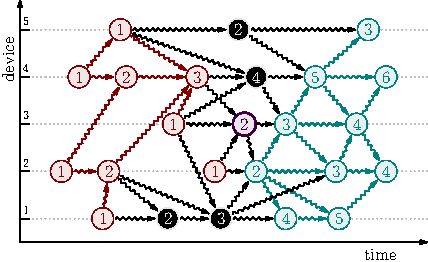
\includegraphics[width=0.8\textwidth]{imgs/structure.pdf}	
\caption{Example of a space-time event structure from \cite{Share}, comprising events (circles), neighbour relations (arrows) and devices (ordinate axis). With respect to the doubly-circled event, the red events are its causal past, the cyan its causal future and the black ones are concurrent.}
\label{fig:eventstructure}
\end{figure}

Figure \ref{fig:eventstructure} shows an example of an event structure, showing the relations among events.

The field calculus is a tiny functional language based on a set of abstract operators for the field computations. In this thesis only an higher-order extension of the field calculus, called \textit{higher-order field calculus (HFC)} \cite{FieldCalculus}, will be considered. HFC extends the field calculus by treating function as first-class values and will be simply refered to as \textit{field calculus} from now on.

\begin{figure}[t]
\centering
\centerline{\framebox[\linewidth]{$
        \begin{array}{lcl@{\hspace{18mm}}r}
                \PROGRAM & \BNFcce & \overline{\FUNCTION}  \; \e
                &{ \mbox{\footnotesize program}}
                \\[3pt]
                \FUNCTION & \BNFcce &  \defK \,\; \fname (\overline{\xname}) \; \{ \e \}
                &{ \mbox{\footnotesize function declaration}}
                \\[3pt]
                \e & \BNFcce &  \xname \;\BNFmid\; \anyvalue \;\BNFmid\; \e(\overline\e) \;\BNFmid\; \fifK (\e) \{\e\} \elseK \{\e\} \;\BNFmid &{ \mbox{\footnotesize expression}} \\
                && \nbrK\{\e\} \;\BNFmid\; \repK(\e)\{ (\xname) \ftoSym \e \} \; \BNFmid \; \\
                && \shareK(\e)\{(\xname) \ftoSym \e \}
                \\[3pt]
                \anyvalue & \BNFcce &  \lvalue \; \BNFmid \; \fvalue
                &{ \mbox{\footnotesize value}}
                \\[3pt]
              \lvalue & \BNFcce &  \dcOf{\dc}{\overline\lvalue} \; \BNFmid \; \funvalue
                &{ \mbox{\footnotesize local value}}
                \\[3pt]
                \fvalue & \BNFcce &  \envmap{\overline\deviceId}{\overline\lvalue}
                &{ \mbox{\footnotesize neighbouring field value}}
                \\[3pt]
                \funvalue & \BNFcce &  \fname \; \BNFmid \; \bname \;\BNFmid\; (\overline{\xname}) \toSym{\name} \e 
                &{ \mbox{\footnotesize function value}}
                \\[3pt]
        \end{array}
        $}
}
\caption{Abstract syntax of the field calculus from \cite{FieldCalculus, Share}} \label{fig:fcsyntax}
\end{figure}

The set of abstract operators is provided in figure \ref{fig:fcsyntax}. Following the notation of \cite{FeatherJava} the overbar denotes a sequence, for example $\overline{\e}$  denotes a (possible empty) sequence of expressions $\e_1, \e_2, \dots, \e_n$.

A program is then a sequence of function definition followed by a main expression $e$, which defines the behavior of the aggregate. 

A function declaration defines a function named $d$ with a sequence of variable names $\overline{\xname}$ and a body of the function consisting in an expression $e$. The defined functions can be recursive.

An expression can be:
\begin{itemize}
\item a variable $\xname$ referring a function parameter
\item a function call $\e(\overline{\e})$, where $\e$ evaluates to a field of functions $\funvalue$, $\overline{\e}$ are the function arguments and evaluates to the function application
\item a {branching expression} $\fifK (\e_0) \{\e_1\} \{\e_2\}$, also called  \textit{domain restriction expression}, its a lazy evaluated expression that divides the computation in two branches: the devices for which $\e_0$ evaluates to $\truevalue$ computes $\e_1$, the devices for which $\e_0$ evaluates to $\falsevalue$ coputes $\e_2$
\item an \textit{$\nbrK$-expression}, also called \textit{neightbouring field construction}, $\nbrK\{\e\}$ which evaluates to a field from neighbouring devices (including the execution device) to their most recent evaluation of the expression $\e$
\item a \textit{$\repK$-expression}, also called \textit{time evolution expression}, $\repK(\e_0)\{ (\xname) \ftoSym \e \}$, which at each round evaluates to the application to the function of the result of the previous round, using the \textit{initialization expression} $\e_0$ in the first round
\item a \textit{$\shareK$-expression} $\shareK(\e_1)\{(\xname) \ftoSym \e_2 \}$, which each round evaluates to the application of the function with the argument $\xname$ taking the value of a field with the last computed values $\e_2$ by each neighbouring device, using $\e_1$ as the initial value for the executing device.
\end{itemize}

A value can be either a \textit{neighbouring field} $\fvalue$ or a \textit{local value} $\lvalue$. Neighbouring field values doesn't appear in the source code but can only be computed dynamically, usually by built-in operators like $\nbrK$.

Local values can be either \textit{data value} $\dcOf{\dc}{\overline\lvalue}$, in which $\dc$ its a data constructor and $\overline \lvalue$ are local value arguments, or a function value $\funvalue$.

A \textit{function value} $\funvalue$ can be a built-in function $\bname$, a declared function $\fname$ or an anonymous function value $(\overline{\xname}) \toSym{\name} \e$  where $\overline{\xname}$ are variable names for the formal parameter, $\e$ is the body of the function and $\name$ is a \texttt{tag} identifying the function. $\name$ doesn't appear in the source code but is uniquely determined by the function syntactical representation.

\section{Field Calculus Semantic}

\begin{figure}[!t]{
 \framebox[1\textwidth]{
 $\begin{array}{l}
 \textbf{Value-trees and value-tree environments:}\\
\begin{array}{lcl@{\hspace{6.8cm}}r}
%
\vtree & \BNFcce &  \mkvt{\anyvalue}{\overline{\vtree}}    &   {\footnotesize \mbox{value-tree}} \\
\Trees & \BNFcce & \envmap{\overline{\deviceId}}{\overline{\vtree}}   &   {\footnotesize \mbox{value-tree environment}}
%
\end{array}\\[10pt]
\hline\\[-8pt]
%%%%  AUX
\textbf{Auxiliary functions:}\\
\begin{array}{l}
\begin{array}{l@{\hspace{1cm}}l}
%
\vrootOf{\mkvt{\anyvalue}{\overline{\vtree}}}  =   \anyvalue
\\
%
\piIof{i}{\mkvt{\anyvalue}{\vtree_1,\ldots,\vtree_n}}  =   \vtree_i
\quad \mbox{if} \; 1\le i \le n
\\
\piBof{\funvalue}{\mkvt{\anyvalue}{\vtree_1,\ldots,\vtree_{n+1}}}  =   \vtree_{n+1}
\quad \mbox{if} \; \funvalue \; \mbox{is a built-in function and} \; \vrootOf{\vtree_{n+1}} = \funvalue
\\
\piBof{\funvalue}{\mkvt{\anyvalue}{\vtree_1,\ldots,\vtree_{n+2}}}  =   \vtree_{n+2}
\quad \mbox{if} \; \funvalue \; \mbox{is a non-built-in function and} \; \nameOf(\vrootOf{\vtree_{n+1}}) = \nameOf(\funvalue)
\\
 \piBof{\funvalue}{\vtree}  =   \emptyseq \quad \mbox{otherwise}
\\  
\end{array}
\\
\mbox{For } \auxNAME\in\rho,\piI{i},\piB{\funvalue}:
\quad 
\left\{\begin{array}{lcll}
 \aux{\envmap{\deviceId}{\vtree}, \Trees}  & =  & \envmap{\deviceId}{\aux{\vtree}}, \aux{\Trees} & \quad \mbox{if} \; \aux{\vtree} \not=\emptyseq  
\\
\aux{\envmap{\deviceId}{\vtree}, \Trees}  & =   & \aux{\Trees} & \quad \mbox{if} \; \aux{\vtree}=\emptyseq  
\\
\aux{\emptyseq}  & =  &  \emptyseq
\end{array}\right.   
\\
\begin{array}{lll}
\nameOf(\fname) = \fname 
& 
\args{\fname} = \overline{\xname} \quad \mbox{if } \, \defK \; \fname (\overline{\xname}) \; \{\e\}
&
\body{\fname} = \e  \quad \mbox{if } \, \defK \; \fname (\overline{\xname}) \; \{\e\}
\\
\nameOf((\overline{\xname}) \toSym{\name} \e) = \name
&
\args{(\overline{\xname}) \toSym{\name} \e} = \overline{\xname}
&
\body{(\overline{\xname}) \toSym{\name} \e} = \e
\end{array}
\\
\begin{array}{l@{\hspace{0.4cm}}l}
		\fvalue_0[\fvalue_1] = \fvalue_2 \; \text{ where } \fvalue_2(\deviceId) = \left\lbrace \begin{array}{ll}
			\fvalue_1(\deviceId) & \text{if } \deviceId \in \domof{\fvalue_1} \\
			\fvalue_0(\deviceId) & \text{otherwise}
		\end{array} \right. \\
\end{array}
\end{array}\\
\hline\\[-10pt]
\textbf{Syntactic shorthands:}\\
\begin{array}{l@{\hspace{5pt}}l@{\hspace{5pt}}l}
\bsopsem{\deviceId}{\piIofOv{\Trees}}{\senstate}{\overline{\e}}{\overline{\vtree}}
&
  \textrm{where~~} |\overline{\e}|=n
&
  \textrm{for~~}
  \bsopsem{\deviceId}{\piIof{1}{\Trees}}{\senstate}{\e_1}{\vtree_1}
    \cdots
    \bsopsem{\deviceId}{\piIof{n}{\Trees}}{\senstate}{\e_n}{\vtree_n} \!\!\!\!\!\!\!\!\!\!\!\! \\
\vrootOf{\overline{\vtree}}
&
  \textrm{where~~} |\overline{\vtree}|=n
  & \textrm{for~~}
\vrootOf{\vtree_1},\ldots,\vrootOf{\vtree_n}\\
\substitution{\overline{\xname}}{\vrootOf{\overline{\vtree}}}
&   \textrm{where~~} |\overline{\xname}|=n
  &
  \textrm{for~~}
\substitution{\xname_1}{\vrootOf{\vtree_1}}~\ldots\quad\substitution{\xname_n}{\vrootOf{\vtree_n}}
\end{array}\\
\hline\\[-10pt]
%%%  EVALUATION RULES
\textbf{Rules for expression evaluation:} \hspace{4.4cm} %\hfill
%\vspace{-0.2cm}
  \boxed{\bsopsem{\deviceId}{\Trees}{\senstate}{\e}{\vtree}}
\skiptransition%[-5pt]
\begin{array}{c}
%\vspace{-0.1cm}
\nullsurfaceTyping{E-LOC}{
\bsopsem{\deviceId}{\Trees}{\senstate}{\lvalue}{\mkvt{\lvalue}{}}
}
\qquad\qquad
\surfaceTyping{E-FLD}{\qquad \fvalue' = \proj{\fvalue}{\domof{\Trees}\cup\{\deviceId\}}}{
\bsopsem{\deviceId}{\Trees}{\senstate}{\fvalue}{\mkvt{\fvalue'}{}}
}
\skiptransition\\[-6pt]
\surfaceTyping{E-B-APP}{  \quad
\begin{array}{c}
  \bsopsem{\deviceId}{\piIofOv{\Trees}}{\senstate}{\overline{\e},\e}{\overline{\vtree},\vtree}
  \qquad \bname=\vrootOf{\vtree}
  \qquad \anyvalue=\builtinop{\bname}{\correction{\deviceId}}{\piBof{\bname}{\Trees},\senstate}(\vrootOf{\overline{\vtree}})
\end{array}
 }{
\bsopsem{\deviceId}{\Trees}{\senstate}{\e(\overline{\e})}{\mkvt{\anyvalue}{\overline{\vtree},\vtree}}
}
%
\skiptransition\\[-6pt]
%
\surfaceTyping{E-D-APP}{ \quad
\begin{array}{c}
  \bsopsem{\deviceId}{\piIofOv{\Trees}}{\senstate}{\overline{\e},\e}{\overline{\vtree},\vtree} \qquad 
  \funvalue=\vrootOf{\vtree} \mbox{is not a built-in} \qquad
\\
  \bsopsem{\deviceId}{\piBof{\funvalue}{\Trees}}{\senstate}{\applySubstitution{\body{\funvalue}}{\substitution{\args{\funvalue}}{\vrootOf{\overline{\vtree}}}}}{\vtree'}
\end{array}
 }{
\bsopsem{\deviceId}{\Trees}{\senstate}{\e(\overline{\e})}{\mkvt{\vrootOf{\vtree'}}{\overline{\vtree},\vtree,\vtree'}}
}
%
\skiptransition\\[-5pt]
\surfaceTyping{E-NBR}{
         \qquad
     \Trees_1=\piIof{1}{\Trees} \qquad
     \bsopsem{\deviceId}{\Trees_1}{\senstate}{\e}{\vtree_1}
\qquad
 \fvalue=\mapupdate{\vrootOf{\Trees_1}}{\envmap{\deviceId}{\vrootOf{\vtree_1}}}
 }{
\bsopsem{\deviceId}{\Trees}{\senstate}{\nbrK\{\e\}}{\mkvt{\fvalue}{\vtree_1}}
}
\skiptransition\\[-6pt]
\surfaceTyping{E-REP}{
        \quad
        \begin{array}{l}
     \bsopsem{\deviceId}{\piIof{1}{\Trees}}{\senstate}{\e_1}{\vtree_1} \\
     \bsopsem{\deviceId}{\piIof{2}{\Trees}}{\senstate}{\applySubstitution{\e_2}{\substitution{\xname}{\lvalue_0}}}{\vtree_2}~~
        \end{array}
        \quad
        \lvalue_0 \! = \!\left\{\begin{array}{ll}
                             \vrootOf{\piIof{2}{\Trees}}(\deviceId) & \mbox{if} \;  \deviceId \in \domof{\Trees} \\
                             \vrootOf{\vtree_{1}} & \mbox{otherwise}
                           \end{array}\right.
 }{
\bsopsem{\deviceId}{\Trees}{\senstate}{\repK(\e_1)\{(\xname) \; \ftoSym \; \e_2\}}{\mkvt{\vrootOf{\vtree_{2}}}{\vtree_1,\vtree_2}}
}
\skiptransition\\[-4pt]
\surfaceTyping{E-IF}{
     \bsopsem{\deviceId}{\piIof{1}{\Trees}}{\senstate}{\e}{\vtree_1}
\qquad
\lvalue_0,\lvalue_1 \! = \!\left\{\begin{array}{ll}
                             \piIof{1}{\Trees},\e_1 & \mbox{if} \;  \vrootOf{\vtree_{1}} = \truevalue\\
                             \piIof{2}{\Trees},\e_2 & \mbox{if} \;  \vrootOf{\vtree_{1}} = \falsevalue
                           \end{array}\right.
\qquad
\bsopsem{\deviceId}{\lvalue_0}{\senstate}{\lvalue_1}{\vtree}
 }{
\bsopsem{\deviceId}{\Trees}{\senstate}{\fifK (\e) \{\e_1\} \{\e_2\}}{\mkvt{\vrootOf{\vtree}}{\vtree_1,\vtree}}
}
\skiptransition\\[-4pt]
\surfaceTyping{E-SHARE}{ \qquad
	\begin{array}{l@{\hspace{0.5em}}l}
     \bsopsem{\deviceId}{\piIof{1}{\Trees}}{{\senstate}}{\e_1}{\vtree_1} & \fvalue' = \vrootOf{\piIof{2}{\Trees}} 
      \qquad \qquad \fvalue = (\envmap{\deviceId}{\vrootOf{\vtree_1}})[\fvalue']
     \\
     \bsopsem{\deviceId}{\piIof{2}{\Trees}}{{\senstate}}{\applySubstitution{\e_2}{\substitution{\xname}{\fvalue}}}{\vtree_2} %& \fvalue = (\envmap{\deviceId}{\vrootOf{\vtree_1}})[\fvalue']
	\end{array}
	\!\!\!\!
 }{
	\bsopsem{\deviceId}{\Trees}{\senstate}{\shareK(\e_1)\{(\xname) \; \ftoSym \; \e_2\}}{\mkvt{\vrootOf{\vtree_{2}}}{\vtree_1,\vtree_2}}
}
\end{array}
\end{array}$}
}
 \caption{Big-step operational semantics adapted from \cite{FieldCalculus}.} \label{fig:deviceSemantics}
\end{figure}

The operational semantics of the syntax is shown in figure \ref{fig:deviceSemantics}. The derive judgements are in the form $\bsopsem{\deviceId}{\Trees}{\senstate}{\e}{\vtree}$ which means that the expression $\e$ evaluates to the value-tree $\vtree$ with respect to the value-tree environment $\Trees$, the device $\deviceId$ and the sensor state $\senstate$. A \textit{value-environment} $\Trees$ is map from device identifies $\deviceId$ to value-trees. A \textit{value-tree} $\vtree$ is an ordered tree of values tracking the results of all the computed subexpressions. The evaluation rules are expressed recursively by evaluating the subexpressions with respect to a new value environment obtained by the subtrees (when present) of the current value-tree environment $\Trees$, this process is called \textit{alignment}. $\senstate$ is a data structure containing information about the device sensors that will be used by the built-in functions.

The auxiliary function $\vroot$ extract the root value of a value-tree, while $\pi$ extracts a subtree from a value-tree. The functions \textit{name}, \textit{args} and \textit{body} extract respectively the name, formal parameters and body of a function.

Rules \ruleNameSize{[E-LOC]} and \ruleNameSize{[E-FLD]} define the evaluation of local values and neighbouring field values. Both produce a value-tree with no subtrees, but in case of neighbouring fields the domain of the field is restrict to the aligned devices.

Rule \ruleNameSize{[E-B-APP]} and \ruleNameSize{[E-D-APP]} model the application of built-in and user-defined (or anonymous) functions. In the first case the root of the value-tree is computed by a function $\builtinop{\bname}{\correction{\deviceId}}{\piBof{\bname}{\Trees},\senstate}$ different for each built-in function $\bname$. In the second case the root is computed by execution the body of the function $\funvalue$, the resulting value-tree also has one additional subtree containing the value-tree resulting from the execution from the body. This is necessary for the alignment of the environment during the execution.

Rule \ruleNameSize{[E-NBR]} models the evaluation of $\mathtt{nbr}$-expression, which extracts from the value-tree environment the neighbouring values to build a neighbouring field as the root result. In the resulting field the value associated with the executing device is updated by the new result of the execution of $\e$.

Rule \ruleNameSize{[E-REP]} models the evaluation of $\mathtt{rep}$-expression, which extract from the value-tree environment the root of the last computed tree in order to replace $\xname$ in the new evaluation of $\e_2$.

Rule \ruleNameSize{[E-IF]} models a branching expression by computing and aligning on only one subtree according to the evaluation of $\e$. This rule is actually not necessary since every $\mathtt{if}$ expression can be rewritten by using the built-in operator $\mathtt{mux}(\e,\e_1,\e_2)$ which eagerly evaluates both $\e_1$ and $\e_2$ and returns the result of one of them according to the truth value computed by $\e$. Every $\fifK(\e)\{\e_1\}\{\e_2\}$ can be rewritten then as $\mathtt{mux}(\e,()\ftoSym\e_1,()\ftoSym\e_2)()$.

Rule \ruleNameSize{[E-SHARE]} models a $\mathtt{share}$-expression, which collects the neighbouring values of the last computations of the expression to form the field $\fvalue$. In case there is not a value for the device $\deviceId$ the root of the evaluation of $\e_1$ is used. Then $\fvalue$ is substituted to $\xname$ in the evaluation of $\e_2$.

\begin{figure}[!t]{
 \framebox[1\textwidth]{
 $\begin{array}{l}
 %%%  SYNTAX
 \textbf{System configurations and action labels:}\\
\begin{array}{lcl@{\hspace{7.5cm}}r}
%
\Field & \BNFcce &  \envmap{\overline\deviceId}{\overline\Trees}    &   {\footnotesize \mbox{status field}} \\
\Topo & \BNFcce &  \envmap{\overline\deviceId}{\overline\devset}    &   {\footnotesize \mbox{topology}} \\
\Sens & \BNFcce &  \envmap{\overline\deviceId}{\overline\senstate}    &   {\footnotesize \mbox{sensors-map}} \\
\Envi & \BNFcce &  \EnviS{\Topo}{\Sens}    &   {\footnotesize \mbox{environment}} \\
\Cfg & \BNFcce &  \SystS{\Envi}{\Field}    &   {\footnotesize \mbox{network configuration}} \\
\act & \BNFcce &  \deviceId \;\BNFmid\; \envact    &   {\footnotesize \mbox{action label}} \\
%
\end{array}\\
\hline\\[-8pt]
\textbf{Environment well-formedness:}\\
\begin{array}{l}
%
\wfn{\EnviS{\Topo}{\Sens}} \textrm{~~holds iff {$\domof{\Topo}=\domof{\Sens}$ and $\Topo(\deviceId) \subseteq \domof{\Sens}$ for all $\deviceId \in \domof{\Sens}$.}}
\\
\end{array}\\
\hline\\[-8pt]
%%%%%%%%%%
%%%  REDUCTION RULES
\textbf{Transition rules for network evolution:} \hfill
  \boxed{\nettran{\Cfg}{\act}{\Cfg}}
  \\[0.2cm]
\vspace{0.5cm}
\begin{array}{c}
\netopsemRule{N-FIR}
                 {\quad \Envi=\EnviS{\Topo}{\Sens}
                   \quad \Topo(\deviceId)= \overline\deviceId 
                  \quad {\bsopsem{\deviceId}{\filter(\Field)(\deviceId)}{\Sens(\deviceId)}{\emain}{\vtree}}
                  \quad
                 \Field_1=\envmap{\overline\deviceId}{\{\envmap{\deviceId}{\vtree}\}}}
                 {\nettran{\SystS{\Envi}{\Field}}{\deviceId}{\SystS{\Envi}{\mapupdate{\filter(\Field)}{\Field_1}}}%\nopsem{\EnviS{\Topo}{\Sens}}{\Field}{\deviceId}{\mapupdate{\Field}{\deviceId}{\vtree}}
                 }
\skiptransition
\netopsemRule{N-ENV}
                 {\qquad \wfn{\Envi'}\qquad \Envi'=\EnviS{\Topo}{\envmap{\overline\deviceId}{\overline\senstate}} \qquad
                  %\bsopsem{\senstate_1}{\emptyset}{\emain}{\vtree_1}\quad\cdots\quad\bsopsem{\senstate_n}{\emptyset}{\emain}{\vtree_n} \qquad
                  \Field_0=\envmap{\overline\deviceId}{\emptyset}
                 }
                 {\nettran{\SystS{\Envi}{\Field}}{\envact}{\SystS{\Envi'}{\mapupdate{\Field_0}{\Field}}}
                 }\\[-10pt]
\end{array}\\
%\textbf{Initial device state $\initialvtree$:}\\[0.2cm]
%\begin{array}{c}
%
%\qquad\qquad\netopsemRule{Init}
%                 {\senstate_0(\snsname)=\initialOf{\typeof{\snsname}}}
%                 {\bsopsem{\senstate_0}{\emptyset}{\emain}{\initialvtree}}
%
%\end{array}
%
\end{array}$}
} %%%\capskip
 \caption{Small-step operational semantics for network evolution from \cite{FieldCalculus}.} \label{fig:networkSemantics}
\end{figure}

Figure \ref{fig:networkSemantics} defines the operational semantics for the evaluation of whole networks, i.e. it models the distributed evolution of the computational fields over time. $\Field$ is map from device identifiers to value-tree environments, modelling the overhall status of the devices at a given time. $\Topo$ models the topology of the network as a map from device identifiers to sets of identifiers of the neigbouring devices. $\Sens$ models the sensors state as map from device identifiers to the local sensor state of the device. $\Envi$ is a couple of topology and sensor state modelling the system's environment. $\Cfg$ models the whole network configuration as a couple of an environment $\Envi$ and a status field $\Field$.

The network semantics is given in terms of small-steps transitions of the king $\nettran{\Cfg}{\act}{\Cfg'}$ where $\act$ can be either a device identifier $\deviceId$ representing its firing or the label $\envact$ representing any environment change. The following notation is used.  $\filter(\cdot)$ is a filtering operation that clears old stored values from the value-tree environements in $\Field$, usually based on space/time tags attached to value-trees. $\envmap{\overline\deviceId}{\Trees}$ denote the map sending each device identifier in $\overline\deviceId$ to the same value-tree environment $\Trees$. $\mapupdate{\Trees_0}{\Trees_1}$ denote the value-tree environment with domain $\domof{\Trees_0} \cup \domof{\Trees_1}$ coinciding with $\Trees_1$ in the domain of $\Trees_1$ and with $\Trees_0$ otherwise. $\Field_0[\Field_1]$ denotes the status field with the same domain as $\Field_0$ made of $\envmap{\deviceId}{\mapupdate{\Field_0(\deviceId)}{\Field_1(\deviceId)}}$ for all $\deviceId$ in the domain of $\Field_1$, $\envmap{\deviceId}{\Field_0(\deviceId)}$ otherwise.

Rule \ruleNameSize{[N-FIR]} models a computational round at a device $\deviceId$. From the filtered local value-tree environement $\filter(\Field)(\deviceId)$ determines the single device semantics obtaining the value-tree $\vtree$ and use it to update the value-tree environment of $\deviceId$'s neighbours.

Rule \ruleNameSize{[N-ENV]} models a change of the environment $\Envi$ to a new well-formed environment $\Envi'$. The devices not appearing in the new environment are removed from the status field and new devices are mapped to the empty context.


\section{Aggregate Programming Layers}

TODO add figure

From the field calculus the aggregate programming framework is built as a series of layers, visibles in figure TODO. The \textit{resilient coordination operators layer} defines using the operators of the field calculus a series of functions that hide the complexity of the basic operators and restric the language to a self-stabilising fragment  of the field calculus \cite{SelfStabilizing}. Then over this operators aggregate programming libraries provides reusable and flexible high level developer APIs, e.g. function for broadcasting values, to computed distances among devices, etc. The application code is then developed on the reusable blocks provided by the libraries.

The resilient coordination layer defines in particular the following three operators:
\begin{itemize}
\item \textit{Block} $\mathtt{G(source, initial, metric, accumulate)}$, a spreading operator for distance measurement and broadcast of values. It computes the shortest-path from a $\mathtt{source}$ (field with value $\truevalue$ for sources) accourting to a $\mathtt{metric}$ (function mapping neightbours to distance) and propagate values up the gradient starting with the value of $\mathtt{initial}$ and accumulating with the binary function $\mathtt{accumulate}$
\item \textit{Block} $\mathtt{C(potential, local, null, accumulate)}$, an operator that accumulates values with the binary function $\mathtt{accumulate}$ down to the $\mathtt{source}$ following the $\mathtt{potential}$ field. $\mathtt{null}$ provides the idempotent value for the accumulation function, $\mathtt{local}$ is accumulated with any values from neighbours at higher potential
\item \textit{Block} $\mathtt{T(initial, zero, decay)}$, a flexible countdown operator starting from $\mathtt{initial}$ to $\mathtt{zero}$ decreasing by the $\mathtt{decay}$ function.
\end{itemize}

Those operators are able to cover many of the common patterns and define a self-stabilising fragment of the field calculus. A computation is self-stabilizing if from any state, without changes of any environment, the computation reaches after a certain number of round a correct final result.


\chapter{Protelis}\label{chap:protelis}

Protelis \cite{Protelis} is a Domain Specific Language providing a practical implementation of the aggregate programming paradigm. It runs on the Java Virtual Machine (JVM) and provides full interoperability with the Java type-system and API. The text Protelis programs are translated into a valid representation of the higher order field calculus semantics, then this representation is executed at regular intervals by the Protelis interpreter. Protelis abstracts over the device capabilities and communication system, allowing to use it for both simulations (like the Alchemist simulator \cite{Alchemist}) and real world application. Protelis also provides a rich standard library for the application developers.

\begin{figure}[t]
\centering
\centerline{$
        \begin{array}{lcl@{\hspace{18mm}}r}
                \PROGRAM & \BNFcce & \overline{\IMPORT} \; \overline{\FUNCTION}  \; \overline{\mathtt{s}};
                &{ \mbox{\footnotesize Program}}
                \\[3pt]
                \IMPORT & \BNFcce & \mathtt{import} \; \iname \;  \BNFmid \; \mathtt{import \; m.*} 
                &{ \mbox{\footnotesize Java import}}
                \\[3pt]
                \FUNCTION & \BNFcce &  \defK \,\; \mathtt{f} (\overline{\xname}) \; \{ \overline{\mathtt{s}} \}
                &{ \mbox{\footnotesize Function definition}}
                \\[3pt]
                \mathtt{s} & \BNFcce &  \e \;\BNFmid\; \mathtt{let} \; \xname \; = \; \e \;\BNFmid \; \xname \; = \; \e
                &{ \mbox{\footnotesize Statement}}
                \\[3pt]
                \mathtt{w} & \BNFcce &  \xname \;\BNFmid\; \mathtt{l} \; \BNFmid \; [\overline{\mathtt{w}}] \;\BNFmid \; \mathtt{f} \; \BNFmid \; (\overline{\xname}) \texttt{->} \{ \; \overline{\mathtt{s}};\}
                &{ \mbox{\footnotesize Variable/Value}}
                \\[3pt]
                \e & \BNFcce &  \mathtt{w} \; \BNFmid \; &{ \mbox{\footnotesize Expression}} \\
	     && \mathtt{b}(\overline{\e}) \; \BNFmid\; \mathtt{f}(\overline{\e}) \;\BNFmid\; \e.\mathtt{apply}(\overline{\e}) \;\BNFmid &{ \mbox{\footnotesize Fun/Op Calls}} \\
                && \e.\mathtt{m}(\overline{\e}) \;\BNFmid\; \texttt{\#}\mathtt{a}(\overline{\e})  \;\BNFmid &{ \mbox{\footnotesize Method Calls}} \\
                && \repK(\xname\texttt{<-}\mathtt{w})\{ \overline{\mathtt{s}};\}  \;\BNFmid &{ \mbox{\footnotesize Persistent state}} \\
                && \mathtt{if}(\e)\{\overline{\mathtt{s}};\}\mathtt{else}\{\overline{\mathtt{s}}';\}  \;\BNFmid &{ \mbox{\footnotesize Exclusive branch}} \\
                && \mathtt{mux}(\e)\{\overline{\mathtt{s}};\}\mathtt{else}\{\overline{\mathtt{s}}';\} \; \BNFmid &{ \mbox{\footnotesize Inclusive branch}} \\
                && \nbrK\{\overline{\mathtt{s}}';\} &{ \mbox{\footnotesize Neighbourhood values}}
                \\[3pt]
        \end{array}
        $
}
\caption{Abstract syntax of the Protelis language from \cite{Protelis}} \label{fig:protelissyntax}
\end{figure}

Figure \ref{fig:protelissyntax} shows the abstract syntax of the Protelis syntax. A Protelis program is composed by a sequence of Java imports, followed by a sequence of function declarations and a sequence of statements composing the main code. Each import specifies the package (if any) and the method name. Each function definition declares a function named $\mathtt{f}$ with a sequence of variables named $\overline{\xname}$ and the body composed by a sequence of statements $\overline{\mathtt{s}}$. The result of a sequence of statements is always considered the value of the last statement of the sequence.


A statement can be an expressions $\e$, a local variable declaration in the form $\mathtt{let} \; \xname \; = \; \e$ where $\xname$ is the new variable name and $\e$ is the expression computing the initial value of the variable, or a re-assignment of a new value to a variable in the form $\xname \; = \; \e$ where $\xname$ is the name of an existing variable and $\e$ is the expression computing the new value.

A value can be a variable name $\xname$, a literal value $\mathtt{l}$ (Boolean, numerical, string), a tuple of values in the form $[\overline{\mathtt{w}}]$, a function name $\mathtt{f}$ or a lambda (i.e. an anonymous function) in the form $ (\overline{\xname}) \texttt{->} \{ \; \overline{\mathtt{s}};\}$ where $\overline{\xname}$ are the arguments and the body is a sequence of statements $\overline{\mathtt{s}}$.

Finally an expression can be:
\begin{itemize}
\item a value $\mathtt{w}$
\item a function call with the arguments $\overline{\e}$, the function can be either a built-in function $\mathtt{b}$\footnote{some built-in function can be called with an infix-style but the syntax has been omitted for simplicity}, a user defined function $\mathtt{f}$ or the application of the argument to a lambda or function name resulting from the evaluation of $\e$
\item a Java method call with the arguments $\overline{\e}$, it can be calling either a method $\mathtt{m}$ on an object computed by $\e$ or a static method via an alias $\#\mathtt{a}$. The aliases are created automatically from the imports.
\item a $\mathtt{rep}$-construct $\repK(\xname\texttt{<-}\mathtt{w})\{ \overline{\mathtt{s}};\}$, equivalent to the field calculus $\mathtt{rep}$, declaring a variable $\xname$ inizialized at $\mathtt{w}$ and updated each round with the result of the execution of the body $\overline{\mathtt{s}}$
\item an $\mathtt{if}$-construct $\mathtt{if}(\e)\{\overline{\mathtt{s}};\}\mathtt{else}\{\overline{\mathtt{s}}';\}$, equivalent to the field calculus $\mathtt{if}$, executing only $\overline{\mathtt{s}}$ or $\overline{\mathtt{s}}'$ according to the branching condition computed by $\e$
\item a $\mathtt{mux}$-construct $\mathtt{mux}(\e)\{\overline{\mathtt{s}};\}\mathtt{else}\{\overline{\mathtt{s}}';\}$, computing both branches $\overline{\mathtt{s}}$ and $\overline{\mathtt{s}}'$ and return the value of one of them accourding to the branching condition computed by $\e$
\item a $\mathtt{nbr}$-construct $\nbrK\{\overline{\mathtt{s}}';\}$, equivalent to the field calculus $\mathtt{nbr}$, returning a field from all neighbors to their last value from computing $\overline{\mathtt{s}}$.
\end{itemize}

\begin{figure}[t]
\begin{lstlisting}[language={Protelis},frame=single,
  emph={count, maxh, distanceTo, distanceToWithObstacle}
]
def count() { rep(x <- 0){ x + 1 } }
def maxh(field) { maxHood(nbr{field}) }
def distanceTo(source) {
  rep(d <- Infinity) {
    mux (source) { 0 }
    else { minHood(nbr{d} + nbrRange) }
  }
}
def distanceToWithObstacle(source, obstacle) {
  if (obstacle) { Infinity } else { distanceTo(source) }
}
\end{lstlisting}
\caption{Examples of Protelis code from \cite{Protelis}}\label{fig:protelisexample}
\end{figure}

Figure \ref{fig:protelisexample} shows an example of Protelis code. The function $\mathtt{count}$ yields the number of round that have been executed. The function $\mathtt{maxh}$ yield a the maximum value of $\mathtt{field}$ across all neighbours using the built-in function $\mathtt{maxHood}$, which takes a field as argument an returns the maximum value. Its important to note that the only way to extract a regular value from a field in Protelis is to use one of the many built-in "hood" functions. The function $\mathtt{distanceTo}$ computes the distance from the device to the nearest device where $\mathtt{source}$ holds $\mathtt{True}$, each device starts with an infinite distance and each round returns zero if it is a source otherwise returns the minimum of the distances shared by the neightbours summed to the distance to that neighbour. It uses the built-in functions $\mathtt{minHood}$ and $\mathtt{nbrRange}$, the former returning the minimum value in the field and the latter returning a field of the distances to each neightbour. The last function $\mathtt{distanceToWithObstacle}$ splits the network in two sub-regions, the normal nodes simply computes the function $\mathtt{distanceTo}$ while the nodes where obstacle holds $\mathtt{True}$ don't partecipate in the algorithm and return an infinite distance.

\chapter{\Scafi{}}\label{chap:scafi}

\Scafi{} \cite{ScafiFirst, Scafi} is a library defining a Domain Specific Language that integrates the aggregate paradigm into the Scala programming language \cite{Scala}. Like Protelis it runs on the Java Virtual Machine but instead of defining its own language it take advantage of the Scala language and its expressive type system. \Scafi{} unlike the others aggregate programming implementation doesn't have an explicit representation of fields but instead has a notion of "computation against a neighbour", i.e. a computation depending on the evaluation of the same expression by an alligned neighbour. This difference aims to provide an embedding of field computations into Scala more close to the host language. It also provides an integration with Akka \cite{Akka}, a Scala industry-ready actor framework for scalable and resilient message-driven applications.

\Scafi{} is an \textit{internal DSL} which means it provides its API on top of the host programming language, unlike Protelis which is an \textit{external DSL}, offering a standalone language. This means that developers doesn't need to learn a new language and the \Scafi{} mantainers don't need to develop editing tools, reusing instead the ones for the Scala language. There is also experimental evidence that Protelis programs require to delegate a significant part of the code to Java methods for code reuse or simplicity. This increases the complexity of development since the code in both languages must be kept coordinated.

\begin{figure}[t]
\begin{lstlisting}[language={scafi},frame=single]
trait Constructs {
  // Key constructs
  def rep[A](init: => A)(fun: (A) => A): A
  def foldhood[A](init: => A)(aggr: (A, A) => A)(expr: => A): A
  def nbr[A](expr: => A): A
  def @@[A](b: => A): A

  // Abstract types
  type ID
  type LSNS, NSNS

  // Contextual, but foundational
  def mid(): ID
  def sense[A](name: LSNS): A
  def nbrvar[A](name: NSNS): A
}
\end{lstlisting}
\caption{\Scafi{} constructs from \cite{Scafi}}\label{fig:scaficonstructs}
\end{figure}

A \Scafi{} program is a function that extends an implementation of the trait $\mathtt{Constructs}$, visible in figuera \ref{fig:scaficonstructs}, which provides all the aggregate programming basic constructs. 

The method $\mathtt{rep}[\mathtt{A}](\mathtt{init}: \texttt{=>} \mathtt{A})(\mathtt{fun}: (\mathtt{A}) \texttt{=>} \mathtt{A}): \mathtt{A}$ implements a $\mathtt{rep}$-expression of the field calculus, returning a value of type $\mathtt{A}$. $\mathtt{init}$ is a lazy expression computing the beginning value. At each round the $\mathtt{fun}$ unary function is applied to compute the new returned value from the last value.

The method $\mathtt{fooldhood}[\mathtt{A}](\mathtt{init}: \texttt{=>} \mathtt{A})(\mathtt{aggr}: (\mathtt{A},\mathtt{A}) \texttt{=>} \mathtt{A})](\mathtt{expr}: \texttt{=>} \mathtt{A}): \mathtt{A}$ provides a way to extract and combine information from neightbours. First the lazy expression $\mathtt{expr}$ is computed against each aligned neighbour, each computation producing a value of type $\mathtt{A}$. Then the results are combined into a single value using the associative binary function $\mathtt{aggr}$ with his neutral element $\mathtt{init}$.

The method $\mathtt{nbr}[\mathtt{A}](\mathtt{expr}: \texttt{=>} \mathtt{A}): \mathtt{A}$ defines a neighbour dependent expression that returns a value of type $\mathtt{A}$. The result is computed by the lazy expression $\mathtt{expr}$ when evaluated against the local device. When evaluated against a neighbouring device it returns instead the most recent value of $\mathtt{expr}$ computed by that device.

The method $@@[\mathtt{A}](\mathtt{b}: \texttt{=>} \mathtt{A}): \mathtt{A}$ is a function that performs an alignment, allowing to perform branching in the execution. Inside the body $\mathtt{b}$ only the neightbours executing the same body are considered aligned. For example the $\mathtt{branch}$ method $\mathtt{branch}[\mathtt{A}](\mathtt{cond}: \mathtt{Boolean})(\mathtt{th}: \texttt{=>} \mathtt{A})(\mathtt{el}: \texttt{=>} \mathtt{A}): \mathtt{A}$, corresponding to the $\mathtt{if}$ in the field calculus, is defined as $\mathtt{mux}(\mathtt{cond})(()\toSymK{\mathtt{th}})(()\toSymK{\mathtt{el}})()$ where $\mathtt{mux}$ is an eagerly evaluated version of the Scala $\mathtt{if}$.

Finally $\mathtt{mid}$ returns the unique identifier, of the abstract type $\mathtt{ID}$, of the running device, $\mathtt{sense}$ reads from the local sensor named $\mathtt{name}$, of the abstract type $\mathtt{LSNS}$, its current value of type $\mathtt{A}$ and $\mathtt{nbrvar}$ reads from a neighbouring sensor named $\mathtt{name}$ (a sensor of the running device which value dependens on the neighbour against which is currently computing), of the abstract type $\mathtt{NSNS}$, its current value of type $\mathtt{A}$. The device temperature or GPS position are examples of local sensors, while the distance from a neighbour is an example of a neighbouring sensor.

\begin{figure}[t]
\begin{lstlisting}[language={scafi},frame=single,emph={count, maxh}]
def count(): Int = { rep(0){ x => x + 1} }
def countNeighbours(): Int = {
  foldhood(0)(_ + _)(1)
}
def maxh(field: Double): Double = { 
  foldhood(Double.NegativeInfinity)(Math.max(_,_)){ nbr(field) } 
}
\end{lstlisting}
\caption{Examples of \Scafi{} programs}\label{fig:scafiexample}
\end{figure}

Figure \ref{fig:scafiexample} shows some example of \Scafi{} programs. The first function $\mathtt{count}$ counts the number of rounds executed by the device. The function $\mathtt{countNeighbours}$ counts how many neighbours has the device, simply by adding one for each device. The function $\mathtt{maxh}$ returns the maximum value $\mathtt{field}$ with which is called across neighbours. This is accomplished by calling $\mathtt{nbr}$ against each neighbour and combining the values by the Scala $\mathtt{Math.max}$ function.

\chapter{Differences between \Scafi{} semantics and field calculus}\label{chap:comparison}

\section{\FSCAFI{} semantic}

Since \Scafi{} is based on the notion of computations against a neighbour instead of neighbouring values it has different semantics from the higher order field calculus (\HFC) and its implementation Protelis. In order to formalize the semantic of \Scafi{} a subset of it has been considered called \textit{Featherweight \Scafi{} (\FSCAFI)} \cite{Scafi} and only the semantic of \FSCAFI has been considered. It has been proved that both \FSCAFI and \HFC{} can express programs that the other can't, but they have a non-empty intersection that can express all the self-stabilising build blocks.

\begin{figure}[t]
\centering
\centerline{$
\begin{array}{l@{\hspace{1mm}}c@{\hspace{1mm}}l@{\hspace{-8mm}}r}
        \PROGRAM & \BNFcce & \overline{\FUNCTION}  \; \e
                                                                                                                                                                                                        &   {\footnotesize \mbox{program}} \\[3pt]
        \FUNCTION & \BNFcce &  \defK \; \fname (\overline{\xname}) \; \eqSymK{\e}
                                                                                                                                                                                                        &   {\footnotesize \mbox{function declaration}} \\[3pt]
        \e & \BNFcce & \xname \, \BNFmid \, \anyvalue \, \BNFmid \, \e(\overline{\e}) \, \BNFmid \, \repK(\e)\{ \e \} \, \BNFmid \, \nbrK\{\e\} \, \BNFmid \, \foldK(\e)(\e)\{\e\} \,
                                                                                                                                                                                                        &   {\footnotesize \mbox{expression}} \\[3pt]
        \hline \\[-6pt]
        \anyvalue & \BNFcce &  {\dc(\overline{\anyvalue})} \; \BNFmid \; \funvalue
                                                                                                                                                                                                        &   {\footnotesize\mbox{value}} \\
        \funvalue & \BNFcce & \bname \; \BNFmid \; \fname \; \BNFmid \; (\overline{\xname}) \; \toSymKtag{\name}{\e}
                                                                                                                                                                                                        &   {\footnotesize\mbox{function value}} \\
\end{array}
$
}
\caption{Syntax of \FSCAFI{} from \cite{Scafi}}
\label{fig:fscafisyntax}
\end{figure}

The syntax of \FSCAFI is shown in figure \ref{fig:fscafisyntax}, it focus on the aggregate constructs ignoring the Scala specific features. A program $\PROGRAM$ is defined as a sequence of function declarations $\overline{\FUNCTION}$ followed by a main expression $\e$. A function declaration $\FUNCTION$ defines a (possibly recursive) function named $\fname$, with a sequence of formal parameters $\overline{\xname}$ and a body expression $\e$. An expression can be a variable $\xname$, a value $\anyvalue$, a function call $\e(\overline{\e})$ where $\e$ evaluates to a function $\funvalue$ and $\overline{\e}$ are the arguments, a $\mathtt{rep}$-expression $\repK(\e)\{ \e \}$ modelling time evolution, a $\mathtt{nbr}$-expression $\nbrK\{\e\}$ modelling neighbourhood interaction or a $\mathtt{foldhood}$-expression $\foldK(\e)(\e)\{\e\}$ combaining a computation against neighbours.

A value can be either a \textit{data value} $\dc(\overline{\anyvalue})$ consisting of a \textit{data constructor} $\dc$ applied to a sequence of values $\overline{\anyvalue}$, or a \textit{function value} $\funvalue$. A function value can be the name of a built-in function $\bname$, the name of a user defined function $\fname$, or an anonymous function $(\overline{\xname}) \; \toSymKtag{\name}{\e}$ where $\overline{\xname}$ are the formal parameters, $\e$ the body of the function and $\name$ a \textit{tag} that uniquely identifies the function and doesn't occours in the source program. A built-in function can be a \textit{pure operator} like the $\mathtt{mux}$ function or mathematical operators, a \textit{sensor} which depends on the environmental conditions of the computing device, or a \textit{relational sensor} which is a sensor depending additionally on a neighbouring device which the computation is happening against.

\begin{figure}[!t]{
 $\begin{array}{l}
\textbf{Value-trees  
and value-tree environments:}\\
\begin{array}{rcl@{\hspace{8.1cm}}r}
	\vtree & \BNFcce &  \mkvtree{E-Rule}{\anyvalue}{\overline{\vtree}}   
	&   {\footnotesize \mbox{value-tree}} \\
	\Trees & \BNFcce & \envmap{\overline{\deviceId}}{\overline{\vtree}} 
	 &   {\footnotesize \mbox{value-tree environment}} \\
\end{array}\\
\hline\\[-8pt]
\textbf{Auxiliary functions:}\\
\begin{array}{l}
\begin{array}{l@{\hspace{8pt}}l@{\hspace{8pt}}l}
	\nameOf((\overline{\xname}) \; \toSymKtag{\name}{\e}) = \name
	&
	\args{ (\overline{\xname}) \; \toSymKtag{\name}{\e}} = \overline{\xname}
	&
	\body{(\overline{\xname}) \; \toSymKtag{\name}{\e}} = \e
	\\
	\nameOf(\fname) = \fname
	&
	\args{\fname} = \overline{\xname}
	&
	\body{\fname} = \e  \; (\text{if } \, \defK \; \fname (\overline{\xname}) \; \eqSymK{\e})
	\\
	\nameOf(\bname) = \bname
	&
	\vrootOf{\mkvtree{}{\anyvalue}{\overline{\vtree}}}  =   \anyvalue
	\\
	\piIof{i}{\mkvtree{E-Rule}{\anyvalue}{\vtree_1,\ldots,\vtree_n}}  =  \vtree_i
	&
	\text{if~} 1\le i \le n
	&
	\text{~else~} \emptyseq
	\\
	\piBof{\funvalue}{\mkvtree{E-Rule}{\anyvalue}{\vtree_1,\ldots,\vtree_{n+2}}}  =   \vtree_{n+2}
	&
	\text{if~} \nameOf(\vrootOf{\vtree_{1}}) = \nameOf(\funvalue)
	&
	\text{~else~} \emptyseq
\end{array} \!\!\!\!\!\!\!\!\!\!\!\!\!\!\!
\\[30pt]
\mbox{For } \auxNAME\in\rho,\piI{i},\piB{\funvalue}:
\quad 
\left\{{\begin{array}{lcll}
	 \aux{\emptyseq}  & =  & \emptyseq
	\\
	\aux{\envmap{\deviceId}{\vtree}, \Trees}  & =   & \aux{\Trees}  & \quad \mbox{if} \; \aux{\vtree}=\emptyseq  
	\\
	 \aux{\envmap{\deviceId}{\vtree}, \Trees}  & =  & \envmap{\deviceId}{\aux{\vtree}}, \aux{\Trees} & \quad \mbox{if} \; \aux{\vtree} \not=\emptyseq  
\end{array}}\right.   \!\!\!\!\!\!
\end{array}\\
\hline\\[-10pt]
\textbf{Syntactic shorthands:}\\
\begin{array}{l@{\hspace{11pt}}l@{\hspace{11pt}}l}
\bsopsem{\deviceId,\deviceId'}{\piIofOv{\Trees}}{\senstate}{\overline{\e}}{\overline{\vtree}}
&
  \textrm{where~~} |\overline{\e}|=n
&
  \textrm{for~~}
  \bsopsem{\deviceId,\deviceId'}{\piIof{1}{\Trees}}{\senstate}{\e_1}{\vtree_1}
    \cdots
    \bsopsem{\deviceId,\deviceId'}{\piIof{n}{\Trees}}{\senstate}{\e_n}{\vtree_n} \!\!\!\!\!\!\!\!\!\!\!\! \\
\vrootOf{\overline{\vtree}}
&
  \textrm{where~~} |\overline{\vtree}|=n
  & \textrm{for~~}
\vrootOf{\vtree_1},\ldots,\vrootOf{\vtree_n}\\
\substitution{\overline{\xname}}{\vrootOf{\overline{\vtree}}}
&   \textrm{where~~} |\overline{\xname}|=n
  &
  \textrm{for~~}
\substitution{\xname_1}{\vrootOf{\vtree_1}}~\ldots\quad\substitution{\xname_n}{\vrootOf{\vtree_n}}
\end{array}\\
\hline\\[-10pt]
\textbf{Rules for expression evaluation:} \hfill
 \boxed{\bsopsem{\deviceId,\deviceId'}{\Trees}{\senstate}{\e}{\vtree}}
%
\skiptransitionR
%
\begin{array}{c}
\nullsurfaceTyping{E-VAL}{
\bsopsem{\deviceId,\deviceId'}{\Trees}{\senstate}{\anyvalue}{\mkvtree{}{\anyvalue}{}}
}
%
\skiptransitionN\\
%
\surfaceTyping{E-B-APP}{
\begin{array}{ll}
  \bsopsem{\deviceId,\deviceId}{\piIof{1}{\Trees}}{\senstate}{\e}{\vtree} 
                    &
          \bsopsem{\deviceId,\deviceId'}{\piIof{i+1}{\Trees}}{\senstate}{\e_i}{\vtree_i}  \quad \text{for all}\; i \in 1, \ldots, n
      \\
         \anyvalue=\builtinop{\bname}{\deviceId,\deviceId'}{\piBof{\bname}{\Trees},\senstate}(\vrootOf{\overline{\vtree}})
         &
         (\bname = \vrootOf{\vtree} \text{ is not relational }) \vee (\deviceId' \in \domof{\piBof{\bname}{\Trees}} \cup \{\deviceId\})
\end{array} \!\!\!\!
 }{
\bsopsem{\deviceId,\deviceId'}{\Trees}{\senstate}{\e(\overline{\e})}{\mkvtree{}{\anyvalue}{\vtree,\overline{\vtree},\anyvalue}}
}
%
\skiptransitionN\\
%
\surfaceTyping{E-D-APP}{
\begin{array}{ll}
  \bsopsem{\deviceId,\deviceId}{\piIof{1}{\Trees}}{\senstate}{\e}{\vtree} 
& 
\bsopsem{\deviceId,\deviceId'}{\piIof{i+1}{\Trees}}{\senstate}{\e_i}{\vtree_i} \quad \text{for all}\; i \in 1, \ldots, n
 
\\
  \funvalue = \vrootOf{\vtree} \mbox{ is not a built-in}
 & 
  \bsopsem{\deviceId,\deviceId'}{\piBof{\funvalue}{\Trees}}{\senstate}{\applySubstitution{\body{\funvalue}}{\substitution{\args{\funvalue}}{\vrootOf{\overline{\vtree}}}}}{\vtree'}
\end{array} \!\!\!\!
 }{
\bsopsem{\deviceId,\deviceId'}{\Trees}{\senstate}{\e(\overline{\e})}{\mkvtree{}{\vrootOf{\vtree'}}{\vtree,\overline{\vtree},\vtree'}}
}
%
\skiptransitionN\\
%
\surfaceTyping{E-REP}{
        \begin{array}{ll}
     \bsopsem{\deviceId,\deviceId}{\piIof{1}{\Trees}}{\senstate}{\e_1}{\vtree_1} & \anyvalue_1=\vrootOf{\vtree_{1}}\\
     \bsopsem{\deviceId,\deviceId}{\piIof{2}{\Trees}}{\senstate}{\e_2(\anyvalue_0)}{\vtree_2}~~& \anyvalue_2=\vrootOf{\vtree_{2}}
        \end{array}
        \quad
        \anyvalue_0 = \left\{\begin{array}{ll}
                             \vrootOf{\piIof{2}{\Trees}}(\deviceId) & \mbox{if} \;  \deviceId \in \domof{\Trees} \\
                             \anyvalue_1 & \mbox{otherwise}
                           \end{array}\right.
 }{
\bsopsem{\deviceId,\deviceId'}{\Trees}{\senstate}{\repK(\e_1)\{\e_2\}}{\mkvtree{}{\anyvalue_2}{\vtree_1,\vtree_2}}
}
%
\skiptransitionN\\
%
\surfaceTyping{E-NBR}{
         \quad
        \deviceId \neq \deviceId' \in \domof{\Trees}
\qquad
        \vtree = \Trees(\deviceId')
 }{
\bsopsem{\deviceId,\deviceId'}{\Trees}{\senstate}{\nbrK\{\e\}}{\vtree}
}
\qquad
\surfaceTyping{E-NBR-LOC}{
         \quad
     \bsopsem{\deviceId,\deviceId}{\piIof{1}{\Trees}}{\senstate}{\e}{\vtree}
 }{
\bsopsem{\deviceId,\deviceId}{\Trees}{\senstate}{\nbrK\{\e\}}{\mkvtree{}{\vrootOf{\vtree}}{\vtree}}
}
%
\skiptransitionN\\
%
\surfaceTyping{E-FOLD}{
        \begin{array}{ll}
                \bsopsem{\deviceId,\deviceId}{\piIof{1}{\Trees}}{\senstate}{\e_1}{\vtree^1}
                &
                 \quad
               \bsopsem{\deviceId,\deviceId}{\piIof{2}{\Trees}}{\senstate}{\e_2}{\vtree_0}
                  \qquad
               \funvalue = \vrootOf{\vtree_0}
                 \\
                 \deviceId_1,...\deviceId_n = \domof{\Trees}\cup\{\deviceId\} 
               &
               \quad
               n\ge m\ge 1
                \qquad \deviceId_1 = \deviceId
                \\
                 \bsopsem{\deviceId,\deviceId_i}{\piIof{3}{\Trees}}{\senstate}{\e_3}{\vtree_i}
                &
                \quad
               \text{for all } i \in 1,...,m 
                \\
                \bsopsemFAIL{\deviceId,\deviceId_j}{\piIof{3}{\Trees}}{\senstate}{\e_3}{}
                &
                 \quad
               \text{for all } j \in m+1,...,n 
                \\
                  \bsopsem{\deviceId,\deviceId}{\emptyset}{\senstate}{\funvalue(\vrootOf{\vtree^i}, \vrootOf{\vtree_i})}{\vtree^{i+1}}
                &
                \quad
                \text{for all } i \in 1,...,m
        \end{array}
 }{
\bsopsem{\deviceId,\deviceId'}{\Trees}{\senstate}{\foldK(\e_1)(\e_2)\{\e_3\}}{\mkvtree{}{\vrootOf{\vtree^{m+1}}}{\vtree^1, \vtree_0, \vtree_1}}
}
\end{array}
\end{array}$
} 
\vspace{-0.1cm}
 \caption{Big-step operational semantics for expression evaluation from \cite{Scafi}.} \label{fig:fscafisemantics}
\end{figure}

\begin{figure}[!t]{
 $\begin{array}{l}
\textbf{Auxiliary rules for expression evaluation failure:} \hfill
   %\qquad\qquad\qquad\quad\;\;
    \boxed{\bsopsemFAIL{\deviceId,\deviceId'}{\Trees}{\senstate}{\e}}
\skiptransition
\begin{array}{c}
\surfaceTyping{E-NBR-FAIL}{
    ~~ \quad
    \deviceId \neq \deviceId' \not\in \domof{\Trees}
 }{
	\bsopsemFAIL{\deviceId,\deviceId'}{\Trees}{\senstate}{\nbrK\{\e\}}
}
\skiptransitionN
\\
\surfaceTyping{E-R-APP-FAIL}{
	\begin{array}{ll}
	\bsopsem{\deviceId,\deviceId}{\piIof{1}{\Trees}}{\senstate}{\e}{\vtree} 
      &
      ~
       \bsopsem{\deviceId,\deviceId'}{\piIof{i+1}{\Trees}}{\senstate}{\e_i}{\vtree_i} ~~ \text{for all}\; i \in 1, \ldots, n
      \\
      \snvalue = \vrootOf{\vtree} \mbox{ is a relational-built-in}
      & 
    ~
    \deviceId \neq \deviceId' \not\in \domof{\piBof{\snvalue}{\Trees}}
	\end{array}
 }{
	\bsopsemFAIL{\deviceId,\deviceId'}{\Trees}{\senstate}{\e(\overline\e)}
}
\skiptransitionN
\\
%\surfaceTyping{E-APP-FUN-FAIL}{
%	~~ \quad
%	\bsopsemFAIL{\deviceId,\deviceId}{\piIof{n+1}{\Trees}}{\senstate}{\e}
% }{
%	\bsopsemFAIL{\deviceId,\deviceId'}{\Trees}{\senstate}{\e(\overline\e)}
%}
%\skiptransitionN
%\\
\surfaceTyping{E-APP-ARG-FAIL}{  
	\begin{array}{ll}
	 \bsopsem{\deviceId,\deviceId}{\piIof{1}{\Trees}}{\senstate}{\e}{\vtree}  
       & 
      \quad
       \overline{\e} = \e_1,...,\e_n 
        \qquad
         n\ge 0
	   \\
	  \bsopsem{\deviceId,\deviceId'}{\piIof{i+1}{\Trees}}{\senstate}{\e_i}{\vtree_i}
	&
	  \quad
	               \text{for all } i \in 1,...,m < n
	\\
	  \bsopsemFAIL{\deviceId,\deviceId'}{\piIof{m+2}{\Trees}}{\senstate}{\e_{m+1}}
	\end{array}
 }{
	\bsopsemFAIL{\deviceId,\deviceId'}{\Trees}{\senstate}{\e(\overline{\e})}
}
\skiptransitionN
\\
\surfaceTyping{E-D-APP-FAIL}{
	\begin{array}{ll}
		\bsopsem{\deviceId,\deviceId}{\piIof{1}{\Trees}}{\senstate}{\e}{\vtree} 
       & 
       \quad
       \bsopsem{\deviceId,\deviceId'}{\piIof{i+1}{\Trees}}{\senstate}{\e_i}{\vtree_i} ~~ \text{for all}\; i \in 1, \ldots, n
        \\
        \funvalue = \vrootOf{\vtree} \mbox{ is not a built-in}
        & 
        \quad
	  \bsopsemFAIL{\deviceId,\deviceId'}{\piBof{\funvalue}{\Trees}}{\senstate}{\applySubstitution{\body{\funvalue}}{\substitution{\args{\funvalue}}{\vrootOf{\overline{\vtree}}}}} %\!\!\!\!\!\!\!\!\!
	\end{array}
 }{
	\bsopsemFAIL{\deviceId,\deviceId'}{\Trees}{\senstate}{\e(\overline{\e})}
}
\end{array}
\end{array}$
} 
\vspace{-0.1cm}
\caption{Big-step operational semantics for expression evaluation from \cite{Scafi} (auxiliary rules for expression evaluation failure).} \label{fig:fscafisemanticsFAIL}
\end{figure}


The semantics of \FSCAFI is shown in figure \ref{fig:fscafisemantics}. Like the field calculus sematic it follows the same notation and the result of the execution is a value-tree. It also uses the same ausiliary functions. Unlike the field calculus semantics the expression are evaluated against an additional deviced id $\deviceId'$ which is used by the $\mathtt{foldhood}$-expressions to evaluate against a neighbour.

Rule \ruleNameSize{[E-VAL]} defines the evaluation of a value which produce a simple value-tree with only that value.

Rules \ruleNameSize{[E-B-APP]} and \ruleNameSize{[E-D-APP]} model the application of built-in and user-defined (or anonymous) functions. Like for the field calculus semantic the built-ins evaluation is delegated a specific ausiliary functions different for each built-in that may depend on the neighbour device against which the computation is currently happening. In case of user-defined functions the domain of aligned neighbours is restricted to only the ones that executed the same function thanks to the operator $\piBof{\funvalue}{\Trees}$.

Rule \ruleNameSize{[E-REP]}  models the evaluation of $\mathtt{rep}$-expressions just like the field calculus semantic.

Rules \ruleNameSize{[E-NBR]} and \ruleNameSize{[E-NBR-LOC]} both models the evaluation of $\mathtt{nbr}$-expressions, the former in the case that the computation is currently happening against a neightbour, the latter in case is happening against the executing device. In the first case the computed value is read from the value-tree environment, in the second case is computed recursively.

Rule \ruleNameSize{[E-FOLD]} models the evaluation of $\mathtt{foldhood}$-expressions. The expression $\e_3$ is computed against the executing device and against each network and the computed values are combined with the $\e_2$ function with an empty value-tree environment. For the evaluation of $\mathtt{foldhood}$ an additional set of rules, in figure \ref{fig:fscafisemanticsFAIL}, are required to handle the failures deriving by not aligned devices. The derive judgements for the failure cases are in the form $\bsopsemFAIL{\deviceId,\deviceId'}{\Trees}{\senstate}{\e}$ which means that expression $\e$ evaluation fails on the device $\deviceId$ against neightbour $\deviceId'$ with respect to the value-tree environment $\Trees$ and sensor state $\senstate$. The rule \ruleNameSize{[E-NBR-FAIL]} models the evaluation of an $\mathtt{nbr}$-expression against a non-aligned device, which results in a failure. Rule \ruleNameSize{[E-R-APP-FAIL]} models the failure on the evaluation of a built-in operators which is a relational sensor computing against a non-aligned device. Finally rules \ruleNameSize{[E-APP-ARG-FAIL]} and \ruleNameSize{[E-D-APP-FAIL]} model the propagation of failures when evaluating function application, the former handles failures in the evaluation of the arguments, the latter handles failure in the evaluation of the function.

\begin{figure}[!t]{
 $\begin{array}{l}
 
 \textbf{Network configurations and action labels:}\\
\begin{array}{lcl@{\hspace{7.6cm}}r}
%
\Field & \BNFcce &  \envmap{\overline\deviceId}{\overline\Trees}    &   {\footnotesize \mbox{computational field}} \\
\Topo & \BNFcce &  \envmap{\overline\deviceId}{\overline\devset}    &   {\footnotesize \mbox{topology}} \\
\Sens & \BNFcce &  \envmap{\overline\deviceId}{\overline\senstate}    &   {\footnotesize \mbox{sensors-map}} \\
\Envi & \BNFcce &  \EnviS{\Topo}{\Sens}    &   {\footnotesize \mbox{environment}} \\
\Cfg & \BNFcce &  \SystS{\Envi}{\Field}    &   {\footnotesize \mbox{network configuration}} \\
\act & \BNFcce &  \deviceId \;\BNFmid\; \envact    &   {\footnotesize \mbox{action label}} \\
%
\end{array}\\
\hline\\[-8pt]
\textbf{Environment well-formedness:}\\
\begin{array}{l}
%
\wfn{\EnviS{\Topo}{\Sens}} \textrm{~~holds if $\Topo,\Sens$ have same domain, and $\Topo$'s values do not escape it.}
\\
\end{array}\\
\hline\\[-8pt]
\textbf{Transition rules for network evolution:} \hfill
  \boxed{\nettran{\Cfg}{\act}{\Cfg}}
  \\[0.2cm]
\vspace{0.5cm}
\begin{array}{c}
\netopsemRule{N-FIR}{ \quad
                 \Envi=\EnviS{\Topo}{\Sens}
                   \quad \Topo(\deviceId)= \overline\deviceId 
                  \quad \bsopsem{\deviceId,\deviceId}{\filter_\deviceId(\Field)(\deviceId)}{\Sens(\deviceId)}{\emain}{\vtree}
                  \quad
                 \Field_1=\envmap{\overline\deviceId}{\{\envmap{\deviceId}{\vtree}\}}
                 }{
                 \nettran{\SystS{\Envi}{\Field}}{\deviceId}{\SystS{\Envi}{\mapupdate{\filter_\deviceId(\Field)}{\Field_1}}}
                 }
\skiptransition
\netopsemRule{N-ENV}
                 {\qquad \wfn{\Envi'}\qquad \Envi'=\EnviS{\Topo}{\envmap{\overline\deviceId}{\overline\senstate}} \qquad
                  
                  \Field_0=\envmap{\overline\deviceId}{\emptyset}
                 }
                 {\nettran{\SystS{\Envi}{\Field}}{\envact}{\SystS{\Envi'}{\mapupdate{\Field_0}{\Field}}}
                 }\\[-10pt]
\end{array}\\
%
%
%
\end{array}$
} 
 \caption{Small-step operational semantics for network evolution from \cite{Scafi}.} \label{fig:fscafinetworkSemantics}
\end{figure}

Figure \ref{fig:fscafinetworkSemantics} defines the operational semantics of whole networks. It uses the same syntax of the \HFC{} network semantics and the same rules. 
Rule \ruleNameSize{[N-FIR]} models a computational round on device $\deviceId$ by computing its local semantics on the filtered value-tree environment obtaining a value-tree $\vtree$, which is used to update the network configuration of the neighbours. Rule \ruleNameSize{[N-ENV]} models an environment change from $\Envi$ to a new well-formed environment $\Envi'$, the computational field is updated by removed the devices that are not part of the new environment and assigning an empty context to the new devices.

\section{\FSCAFI{} typing}

\begin{figure}[!t]{
 \scalebox{0.9}{
 $\begin{array}{l}
%%%  TYPES
\textbf{Types:}\\
\begin{array}{rcl@{\hspace{7.5cm}}r}
%
\type & \BNFcce &  \tvar  \; \BNFmid \;  \builtintype \; \BNFmid \;  (\overline\type) \rightarrow \type        &   {\footnotesize \mbox{type}} \\
%
\typescheme & \BNFcce &  \forall\overline{\tvar}.\type      &   {\footnotesize \mbox{type scheme}} \\
%
%\localenv & \BNFcce & \envS{\senstate}{\overline\vtree} &   {\footnotesize \mbox{local environment}} \\
\end{array}\\
\hline\\[-8pt]
%%%  TYPE RULES
\textbf{Expression typing:} 
  \hfill
  \boxed{\expTypJud{\TStypEnv}{\TtypEnv}{\e}{\type}}
\vspace{0.1cm}
  \\
\begin{array}{c}
%
\nullsurfaceTyping{T-VAR}{
\expTypJud{\TStypEnv}{\TtypEnv,\xname:\type}{\xname}{\type}
}
\qquad
%
{
\surfaceTyping{T-DAT}{ \quad
\applySubstitution{\type'}{\substitution{\overline\tvar}{\overline\type''}} = (\overline{\type})\rightarrow\type
\qquad
\expTypJud{\TStypEnv}{\TtypEnv}{\overline{\anyvalue}}{\overline{\type}}
}{
\expTypJud{\TStypEnv,\dc: \forall \overline{\tvar}. \type'}{\TtypEnv}{\dc(\overline{\anyvalue})}{\type} }
}
%
\skiptransition
%
\surfaceTyping{T-A-FUN}{ \quad
\expTypJud{\TStypEnv}{\;\TtypEnv,\,\overline{\xname}:\overline{\type}}{\e}{\type}
}{ \expTypJud{\TStypEnv}{\TtypEnv}{ (\overline{\xname}) \toSymKtag{\name}{\e}}{(\overline{\type})\rightarrow\type} }
%
\qquad
%
{
\surfaceTyping{T-N-FUN}{ \quad
\mbox{$\funvalue$ is a (built-in or declared) function}}{
\expTypJud{\TStypEnv,\funvalue: \forall \overline{\tvar}. \type}{\TtypEnv}{\funvalue}{\applySubstitution{\type}{\substitution{\overline\tvar}{\overline\type}}} }
}
%
\skiptransition
%
%
\surfaceTyping{T-APP}{ \quad
\expTypJud{\TStypEnv}{\TtypEnv}{\e}{(\overline{\type})\rightarrow\type} \qquad
\expTypJud{\TStypEnv}{\TtypEnv}{\overline{\e}}{\overline{\type}} }{
\expTypJud{\TStypEnv}{\TtypEnv}{\e(\overline{\e})}{\type} }
%
\skiptransition
%
%\surfaceTyping{T-BRANCH}{ \qquad
%\expTypJud{\TStypEnv}{\TtypEnv}{\e_1}{\btype}
%\quad \expTypJud{\TStypEnv}{\TtypEnv}{\e_2}{\type}
%\quad \expTypJud{\TStypEnv}{\TtypEnv}{\e_3}{\type} }{
%\expTypJud{\TStypEnv}{\TtypEnv}{\ifK(\e_1) \{\e_2\} \{\e_3\} }{\type} }
%%
%\skiptransition
%%
\surfaceTyping{T-REP}{ \qquad
\expTypJud{\TStypEnv}{\TtypEnv}{\e_1}{\type}
\qquad \expTypJud{\TStypEnv}{\TtypEnv}{\e_2}{(\type)\to \type} }{
\expTypJud{\TStypEnv}{\TtypEnv}{\repK(\e_1)\{\e_2\}}{\type} }
%
\qquad\qquad
%
\surfaceTyping{T-NBR}{ \qquad
\expTypJud{\TStypEnv}{\TtypEnv}{\e}{\type}
}{ \expTypJud{\TStypEnv}{\TtypEnv}{\nbrK\{\e\}}{\type} }
%
\skiptransition
%
\surfaceTyping{T-FOLD}{ \qquad
\expTypJud{\TStypEnv}{\TtypEnv}{\e_1}{\type}
\quad \expTypJud{\TStypEnv}{\TtypEnv}{\e_2}{(\type, \type) \to \type}
\quad \expTypJud{\TStypEnv}{\TtypEnv}{\e_3}{\type} }{
\expTypJud{\TStypEnv}{\TtypEnv}{\foldK(\e_1) (\e_2) \{\e_3\} }{\type} }
%
\skiptransition
%
\end{array}
\\
\textbf{Function typing:} 
  \hfill
  \boxed{\funTypJud{\TStypEnv}{\FUNCTION}{\typescheme}}
  \\
\begin{array}{c}
%
\surfaceTyping{T-FUNCTION}{
\qquad
\expTypJud{\TStypEnv,\,\fname:\forall\emptyseq.(\overline{\type})\rightarrow\type}{\overline{\xname}:\overline{\type}}{\e}{\type}
\qquad
\overline{\tvar}=\FTV{(\overline{\type})\rightarrow\type}
}{ \funTypJud{\TStypEnv}{\defK \; \fname (\overline{\xname}) \; \eqSymK{\e}}{\forall\overline{\tvar}.(\overline{\type})\rightarrow\type}}
%
\skiptransition
%
\end{array}
\\
\textbf{Program typing:} 
  \hfill
  \boxed{\proTypJud{\PROGRAM}{\type}}
  \\
\begin{array}{c}
%
\surfaceTyping{T-PROGRAM}{
\\
\TStypEnv_0=\OStypEnv
\\
\FUNCTION_i = \defK \; \fname_i (\_) \; \eqSymK{\_}
\qquad
\funTypJud{\TStypEnv_{i-1}}{\FUNCTION_i}{\typescheme_i}
\qquad
\TStypEnv_i=\TStypEnv_{i-1},\, \fname_i:\typescheme_i
\qquad
 (i \in 1..n)
\\
\expTypJud{\TStypEnv_n}{\emptyset}{\e}{\type}
}{ \proTypJud{\FUNCTION_1\cdots\FUNCTION_n  \;
\e}{\type}}
\end{array}
\end{array}$}
} \caption{Type rules for \FSCAFI{} expressions, function declarations, and programs. from \cite{Scafi}} \label{fig:fscafiTyping}
\end{figure}

Figure \ref{fig:fscafiTyping} present a type system for \FSCAFI from \cite{Scafi}. A type $\type$ can be either a type variable $\tvar$, a built-in type $\builtintype$ or a function type $(\overline\type) \rightarrow \type$. Type schemes $\typescheme$ can produce regular types $\type$ by replacing the type variables with a type. The typing judgement rules are given in the form $\expTypJud{\TStypEnv}{\TtypEnv}{\e}{\type}$, meaning that $\e$ has type $\type$ under the type-scheme assumptions $\TStypEnv$ and the type assumtions $\TtypEnv$. A type scheme environement $\TStypEnv$ collect the type schemes for built-in constructors, built-in operators and user-defined functions. A type environment $\TtypEnv$ collects the types for program variables. $\OStypEnv$ denotes the distinguished built-in type-scheme environment for built-in constructors and built-in functions. $\FTV{\type}$ denotes the set of type variables occurring in the type $\type$.

Rule \ruleNameSize{[T-VAR]} assigns a type to a variable $\xname$ by looking the type assumptions $\TtypEnv$. Rule \ruleNameSize{[T-DAT]} assigns a type to a data value by extracting the type scheme of the data constructor from the type-scheme environment $\TStypEnv$. Rules \ruleNameSize{[T-A-FUN]} and \ruleNameSize{[T-N-FUN]} assign a type to anonymous function and built-in or declared function names, respectively. Rule \ruleNameSize{[T-APP]} assigns a type to a function application. Rule \ruleNameSize{[T-REP]} assigns a type to a $\mathtt{rep}$-expression, ensuring that the initial value and the domain and range of the body have the same type. Rule \ruleNameSize{[T-NBR]} assings a type to a $\mathtt{nbr}$-expression that has the same type as the expression inside the operator. Rule \ruleNameSize{[T-FOLD]} assigns a type to a $\mathtt{foldhood}$-expression, ensuring that $\e_1$ and $\e_3$ have the same type $\type$ and that $\e_2$ has type $(\type,\type) \to \type$.

Rule \ruleNameSize{[T-FUNCTION]} assigns a type scheme to a user defined function. Rule \ruleNameSize{[M-PROGRAM]} allows to type a program with the type of the main expression by adding to the type-scheme environment the type schemes of all the user defined functions.

\section{\Scafi{} and HFC semantics alignment}

\begin{figure}[!t]
\centering
\centerline{$
\begin{array}{ccc}
\HFC{} && \FSCAFI{} \\
\defK \; \fname (\overline{\xname}) \; \{\e\} &\longleftrightarrow& \defK \; \fname (\overline{\xname}) \; \eqSymK{\e} \\
(\overline{\xname}) \; \toSym{\name} \; \e &\longleftrightarrow& (\overline{\xname}) \; \toSymKtag{\name}{\e} \\
\foldK(\e, \e, \e) &\longleftrightarrow& \foldK(\e)(\e)\{\e\}
\end{array}
$
}
\caption{Informal description of the bidirectional translation between \HFC{} and \FSCAFI{} from \cite{Scafi}.} \label{fig:fscafitranslation}
\end{figure}

A \FSCAFI program can be translated into a \HFC{} program and viceversa following simple translation rules shown in figure \ref{fig:fscafitranslation}, assuming the existence of a $\foldK$ built-in function for HFC equivalent to the $\foldK$ operator of \FSCAFI. Those rules don't preserve type-safety and behavior for all programs, however they are preserved for a fragment of the two languages, called respectively HFC' and \textit{Aligned} \FSCAFI. HFC' is obtained by applying three restriction on how field values can be processed:
\begin{description}
	\item[R1]
	Expressions of neighbouring type can only be aggregated to local values with a $\foldK$ operator if they do not capture variables of neighbouring types; so that, e.g., aggregating arguments of neighbouring type is never allowed.
	\item[R2]
	Functions $\funvalue$ with arguments of neighbouring type have to return a neighbouring type.
	\item[R3]
	Built-in functions need to be pointwise or aggregating on neighbouring values.
\end{description}
The reason behind the first rule are visible in the following example:
\begin{lstlisting}[]
def wrong_avghood(x) = {
  foldhood(0, +, x) / foldhood(0, +, 1)
}
wrong_avghood(nbr{sns-temp()})
\end{lstlisting}
and its translation in  \FSCAFI:
\begin{lstlisting}[]
def wrong_avghood(x) = @@{
  foldhood(0)(+){x} / foldhood(0)(+){1}
}
wrong_avghood(nbr{sns-temp()})
\end{lstlisting}
The \HFC{} program computes the average temperature of neighbours while the \FSCAFI{} program is equivalent to the program $\nbrK\{\texttt{sns-temp}()\}$. In the \FSCAFI program if the computation is happening against a neighbour $\deviceId'$ only that temperature $\mathtt{t}$ is used as argument of the function, then it simply compute $nt/n = t$ where $n$ is the number of neighbours. In \Scafi{} a simple solution to write this program is to make $\xname$ a by-name parameter.

The reason for the the second restriction is exemplified in the following program, in which if and branch are both implemented in terms of the $\mathtt{mux}$ built-in function:
\begin{lstlisting}[]
def wrong_ignore(x) = { 1 }
foldhood(0, +, if (sns-temp() > 0) { wrong_ignore(nbr{sns-temp()}) } { 1 } )
\end{lstlisting}
and its translation in  \FSCAFI{}
\begin{lstlisting}[]
def wrong_ignore(x) = @@{ 1 }
foldhood(0)(+){ branch (sns-temp() > 0) { wrong_ignore(nbr{sns-temp()}) } { 1 } }
\end{lstlisting}
The \HFC{} program computes the number of neighbours while the \FSCAFI{} program in case the executing device has a positive temperatures counts only the number of neighbour with positive temperature since the fooldhood evaluation fail against the others.

The reason behind the third rule is exaplained by considering for example a buil-in function $\mathtt{sorthood}$ which rearranges values $\fvalue(\deviceId)$ in increasing order of neighbour identifiers $\deviceId$. So given a neighbouring value $\fvalue = \envmap{\overline\deviceId}{\overline\lvalue}$ and assuming $\deviceId_1 \leq \ldots \leq \deviceId_n$ it returns a neighbouring value $\fvalue' = \envmap{\deviceId_1}{\lvalue_{\pi_1}}, \ldots, \envmap{\deviceId_n}{\lvalue_{\pi_n}}$. this function is conceivable in \HFC{} but it's impossible to implement in \FSCAFI{}.

Those restriction rules can be formalized in \FSCAFI{} by a new set of more restrictive typing rules, obtaining a fragment of the language called \textit{Aligned} \FSCAFI{}. It can be proved \cite{Scafi} that a well-typed program of one of the fragments can be transformed into a well-type program of the other with the same behavior. It can also be proved that Aligned \FSCAFI{} is Turing universal and all the base programming patterns provided in \cite{SelfStabilizing} for designing self-stabilising applications can be rewritten to fit into the fragment.

\begin{figure}[t!]
\scalebox{0.9}{$\begin{array}{l}
%%%  TYPES
\begin{array}{r@{\hspace{1.0cm}}c}
	\begin{array}{rcl@{\hspace{1cm}}r}
		\multicolumn{4}{l}{\textbf{Types:}} \\[1pt]
		\type	& \BNFcce & \tvar \; \BNFmid \; {\rtype} \; \BNFmid \; \ltype											   &   {\footnotesize \mbox{type}} \\
		\ltype	& \BNFcce & \ltvar \; \BNFmid \; {\stype} \; \BNFmid \; (\overline{\type})\to\ftype	 & {\footnotesize \mbox{local type}} \\
		\rtype	& \BNFcce & \rtvar \; \BNFmid \; \stype \; \BNFmid \; \ftype										  &   {\footnotesize \mbox{return type}} \\
		\stype	& \BNFcce & \stvar \; \BNFmid \; \builtintype \; \BNFmid \; (\overline{\ltype})\to\stype	&   {\footnotesize \mbox{local return type}} \\
		\ftype	& \BNFcce & \ftypeOf{\stype}																							&   {\footnotesize \mbox{field type}} \\[2pt]
		\multicolumn{4}{l}{\textbf{Local type schemes:}} \\[1pt]
		\ltypescheme & \BNFcce & \forall\overline{\tvar}\overline{\ltvar}\overline{\rtvar}\overline{\stvar}.\ltype
																																							  &   {\footnotesize \mbox{local type scheme}} \\
	\end{array}
	&
	{\raisebox{-1.3cm}{
	\begin{tikzpicture}[xscale=1.5,yscale=1.1]
		\draw[ultra thick] (-0.5,0) circle (1cm);
		\draw[ultra thick] (0.5,0) circle (1cm);
		\node[draw,rectangle] (TT) at (0, 1.25) {$\type$};
		\node[draw,rectangle] (LT) at (-1, 0.5) {$\ltype$};
		\node[draw,rectangle] (RT) at (1, 0.5) {$\rtype$};
		\node[draw,rectangle] (ST) at (0, -0.5) {$\stype$};
		\node (B) at (0.1, 0.5) {$\builtintype$};
		\node (TxS) at (0, 0.05) {$(\overline\ltype) \rightarrow \stype$};
		\node (F) at (0.8, -0.4) {$\ftype$};
		\node (TxF) at (-0.95, -0.3) {$(\overline\type) \rightarrow \ftype$};
	\end{tikzpicture}
	}}
\end{array} \\[38pt]
\hline\\[-8pt]
%%%  EXPRESSIONS
\textbf{~~Expression typing:} \hfill \boxed{\expTypJud{\LTStypEnv}{\TtypEnv}{\e}{\type}} \\[5pt]
\quad
\begin{array}{c}
	\nullsurfaceTyping{T'-VAR}{
		\expTypJud{\LTStypEnv}{\TtypEnv, \xname:\type}{\xname}{\type}
	}
	\qquad
	\surfaceTyping{T'-DAT}{ \quad
		\applySubstitution{\stype'}{\substitution{\overline\stvar}{\overline\stype''}} = (\overline{\stype})\rightarrow\stype
		\qquad
		\expTypJud{\TStypEnv}{\TtypEnv}{\overline{\lvalue}}{\overline{\stype}}
	}{
		\expTypJud{\TStypEnv,\dc: \forall\overline\stvar. \stype'}{\TtypEnv}{\dc(\overline{\lvalue})}{\stype}
	}
	\skiptransition
	\surfaceTyping{T'-A-FUN}{  \quad
		\overline{\yname}=\FV{(\overline{\xname}) \; \toSymKtag{\name}{\e}} \quad
		{\expTypJud{\LTStypEnv}{\TtypEnv}{\overline\yname}{\overline{\ltype}}} \quad
		\expTypJud{\LTStypEnv}{\TtypEnv, \overline{\xname} : \overline\type}{\e}{\rtype}
	}{
		\expTypJud{\LTStypEnv}{\TtypEnv}{(\overline{\xname}) \; \toSymKtag{\name}{\e}}{(\overline\type) \rightarrow \rtype}
	}
	\skiptransition
	\surfaceTyping{T'-N-FUN}{ \quad
		\mbox{$\funvalue$ is a (built-in or declared) function}
	}{
		\expTypJud{\TStypEnv,\funvalue : \forall\overline\tvar\overline\ltvar\overline\rtvar\overline\stvar.\ltype}{\TtypEnv}{\funvalue}{\applySubstitution{\ltype}{\substitution{\overline\tvar}{\overline\type},~ \substitution{\overline{\ltvar}}{\overline{\ltype}},~ \substitution{\overline{\rtvar}}{\overline{\rtype}},~ \substitution{\overline{\stvar}}{\overline{\stype}}}}
	}
	\skiptransition
	\surfaceTyping{T'-APP}{ \qquad
		\expTypJud{\LTStypEnv}{\TtypEnv}{\e}{(\overline\type)\rightarrow\rtype} \qquad
		\expTypJud{\LTStypEnv}{\TtypEnv}{\overline{\e}}{\overline\type}
	}{
		\expTypJud{\LTStypEnv}{\TtypEnv}{\e(\overline{\e})}{\rtype}
	}
	\skiptransition
	\surfaceTyping{T'-REP}{ \quad
		\expTypJud{\LTStypEnv}{\TtypEnv}{\e_1}{\stype} \qquad
		\expTypJud{\LTStypEnv}{\TtypEnv}{\e_2}{\stype \rightarrow \stype}
	}{
		\expTypJud{\LTStypEnv}{\TtypEnv}{\repK(\e_1)\{\e_2\}}{\stype}
	}
	\qquad
	\surfaceTyping{T'-NBR}{ \quad
		\expTypJud{\LTStypEnv}{\TtypEnv}{\e}{\stype}
	}{
		\expTypJud{\LTStypEnv}{\TtypEnv}{\nbrK\{\e\}}{\ftypeOf{\stype}}
	}
	\skiptransition
	\surfaceTyping{T'-FOLD}{ \qquad
		\begin{array}{ll}
			\expTypJud{\TStypEnv}{\TtypEnv}{\e_1}{\stype}
			& \quad 
			\expTypJud{\TStypEnv}{\TtypEnv}{\e_3}{\ftypeOf{\stype} \text{ or } \stype}
			\\
			\expTypJud{\TStypEnv}{\TtypEnv}{\e_2}{(\stype, \stype) \rightarrow \stype}
			& \quad 
	        \expTypJud{\TStypEnv}{\TtypEnv}{\overline\xname}{\overline\ltype}
	        \quad\text{where}\; \overline\xname = \FV{\e_3}
		\end{array}
	}{
		\expTypJud{\TStypEnv}{\TtypEnv}{\foldK(\e_1) (\e_2) \{\e_3\} }{\stype}
	}
\end{array} \\~\\
%%%  FUNCTIONS
\textbf{~~Function typing:} \hfill \boxed{\funTypJud{\LTStypEnv}{\FUNCTION}{\ltypescheme}} \\[5pt]
\qquad \qquad
\begin{array}{c}
	\surfaceTyping{T'-FUNCTION}{ \qquad
		\begin{array}{ll}
			\expTypJud{\LTStypEnv, \fname: (\overline\type)\to\rtype}{\overline{\xname}:\overline{\type}}{\e}{\rtype} \qquad
			\overline{\tvar}\overline{\ltvar}\overline{\rtvar}\overline{\stvar}=\FTV{(\overline{\type})\rightarrow\rtype} %\\
			%\text{arguments not occurring in } \e \text{ are local}
		\end{array}
	}{
		\funTypJud{\LTStypEnv}{\defK \; \fname (\overline{\xname}) \; \eqSymK{\e}}{
			\forall\overline{\tvar}\overline{\ltvar}\overline{\rtvar}\overline{\stvar}.(\overline{\type})\rightarrow\rtype
	}}
\end{array} \\~\\
%%%  PROGRAMS
\textbf{~~Program typing:} \hfill {\boxed{\funTypJud{\LTStypEnv_0}{\PROGRAM}{\type}}} \\[5pt]
\qquad \quad
\begin{array}{c}
	\surfaceTyping{T'-PROGRAM}{ \\
		\FUNCTION_i=(\defK \; \fname_i (\_) \; \_) \qquad
		\funTypJud{\LTStypEnv_{i-1}}{\FUNCTION_i}{\ltypescheme_i} \qquad
		\LTStypEnv_i=\LTStypEnv_{i-1},\, \fname_i:\ltypescheme_i \qquad
		(i \in 1..n) \\
		\expTypJud{\LTStypEnv_n}{\emptyset}{\e}{\type}
	}{
		\funTypJud{{\LTStypEnv_0}}{\FUNCTION_1\cdots\FUNCTION_n  \; \e}{{\type}}
	}
\end{array}
\end{array}$}
\caption{Hindley-Milner typing for Aligned \FSCAFI{} expressions, function declarations, and programs. from \cite{Scafi}} \label{fig:alignfscafityping}
\end{figure}

Figure \ref{fig:alignfscafityping} shows the typing rules of aligned \FSCAFI. The types has been divided in four categories, of which only one can appear as a field type from an $\mathtt{nbr}$-expression. The restriction R1 is further implemented by requiring in the rule \ruleNameSize{[T-FOLD]} that each free variable occurring in $\e_3$ has a local type. The restriction R2 is implemented by restricting local function types to $(\overline{\type})\to\ftype$ instead of $(\overline{\type})\to\rtype$. Restriction R3 is implicitly valid for all \FSCAFI programs given the semantic rules.


\chapter{Kotlin}\label{chap:kotlin}

Kotlin \cite{Kotlin} is a general-purpose programming language fully interoperable with Java and developed by JetBrains. Its a cross-platform language, allowing to compile to the JVM, to JavaScript and to native code via LLVM. It supports both the Object-Oriented Programming paradigm and the Functional Programming paradigm. It allows the reuse of Java library on the JVM, its statically typed and supports the definition of custom DSLs. Since May 2017 the Android platform officially supports the Kotlin programming language, with the long term goal of make it the main language for the development of Android applications and libraries.

\section{Class and function definition}

Kotlin is designed to have a syntax familiar to Java developer, like Java it supports the Object-Oriented Programming paradigm. The code is structured in nested packages, each one containing classes and top level functions. Each class :
\begin{itemize}
\item may extend one other class and any number of interfaces
\item may have any number of field, holding values of specified types
\item has one primary constructor, which is responsible of initializing the field, and zero or more secondary constructor which must call the primary constructor
\item may have any number of type parameters, abstracting over the types used inside the class
\item may have any number of functions.
\end{itemize}

The following example shows the definition of a class:
\begin{lstlisting}[language={kotac}]
class Foo<T>(t: T): Serializable {
  var v: T = t
}
\end{lstlisting}
It defines a class named $\mathtt{Foo}$ with a type parameter $\mathtt{T}$ and implementing the Java interface $\mathtt{Serializable}$. The primary constructor takes a single argument $\mathtt{t}$ of type $\mathtt{T}$. A mutable field called $\mathtt{v}$ is declared of type $\mathtt{T}$ and initialized with the value of $\mathtt{t}$.

In Kotlin functions are first class values and function types are directly expressable in the type system. Functions can be defined as class members or as top-level functions. They can have any number of parameters and type parameters. Functions can also be passed as parameters or returned by other functions. Functions can have default arguments, which are parameters with default values. The following example shows the definition of a function:
\begin{lstlisting}[language={kotac}]
fun foo<T>(t: T, i: Int = 0): String { /* ... */ }
\end{lstlisting}
It defines a function named $\mathtt{foo}$ with a type parameter $\mathtt{T}$ that returns a value of type $\mathtt{String}$. It takes one argument of type $\mathtt{T}$ named $\mathtt{t}$ and one argument of type $\mathtt{Int}$ named $\mathtt{i}$ with default value $0$. The body of the function is omitted in the example.

Anonymous functions can be declared as lambdas. A lambda is defined in the following code:
\begin{lstlisting}[language={kotac}]
val foo: (Int) -> String = { i -> i.toString() }
\end{lstlisting}
It defines an immutable variable named $\mathtt{foo}$ which has the type of a function from $\mathtt{Int}$ to $\mathtt{String}$ and its value is the following lambda that returns the string representation of the input.

\section{Kotlin DSLs}

Kotlin has many features that helps design DSLs with robust and type-safe APIs.

Extension functions allows to defines a function as it was a member of an existing class, so that it can be called as it was a member of the original class. Inside the body of the function all the class members (field and functions) are directly accessible.
For example the code:
\begin{lstlisting}[language={kotac}]
fun Int.plusOne(): Int { return this + 1 }
\end{lstlisting}
Declares an extension function of the class $\mathtt{Int}$ named $\mathtt{plusOne}$ that adds one to the integer number on which is called. For instance $4\mathtt{.plusOne()}$ evaluates to $5$.

Trailing lambdas are a syntax feature that allows to write a lambda outside the parentheses when is the last argument of a function allowing write DSLs that can be called with a syntax more similar to built-in constructs. For example the code:
\begin{lstlisting}[language={kotac}]
fun iterate(times: Int, run: () -> Unit) { /* ... */ }
\end{lstlisting}
defines a function named $\mathtt{iterate}$ that can be called like:
\begin{lstlisting}[language={kotac}]
iterate(5) {
  /* ... */
}
\end{lstlisting}

Null safety is a type system feature that allows to write robust APIs. In Kotlin every times a function can accept as argument or return a null value it must be explicitly written in the type signature by adding a "$\mathtt{?}$" to the type. For example the code:
\begin{lstlisting}[language={kotac}]
fun foo(i: Int?): String? { /* ... */ }
\end{lstlisting}
declares a function named $\mathtt{foo}$ with a parameter that can be an instance of $\mathtt{Int}$ or $\mathtt{null}$ and returns a $\mathtt{String}$ or $\mathtt{null}$.


\chapter{\Kotac{}}\label{chap:kotac}

\Kotac{} is an internal Domain Specific Language for the aggregate programming in Kotlin, currently under development at the address \textit{github.com/kklorenzotesta/KotAC}. Its designed to be fully cross-platform with easy to use idiomatic APIs. Like \Scafi{} the internal DSL offers an easy integration with existing code, and the API has the same semantics of the field calculus. It is also designed to be usable for Android applications. The repository has been integrated with the Travis \cite{Travis} continous integration to validate the pushed builds. The library is built with the Gradle \cite{Gradle} build tool, the standard build tool for Kotlin projects, and linted with the ktlint \cite{ktlint} plugin.

\section{Explicit fields}
Unlike \Scafi{}, in which the fields are implicitly represented in the notion of computation against a neighbour, \Kotac{} explicitly represents the field values with the following interface:
\begin{lstlisting}[language={kotac}]
interface Field<out T> {
    fun <R> map(f: (T) -> R): Field<R>
    fun <R> fold(initial: R, operation: (acc: R, T) -> R): R
}
\end{lstlisting}
$\mathtt{Field}$ is an interface with a covariant\footnote{A class or interface $\mathtt{Foo<T>}$ is covariant in $\mathtt{T}$ if, for each class $\mathtt{B}$ subclass of $\mathtt{A}$, $\mathtt{Foo<B>}$ is subclass of $\mathtt{Foo<A>}$} type parameter $\mathtt{T}$, representing the type of the values to which each device in the field is mapped to. A field exposes only two high level functions for its manipulation. The $\mathtt{map}$ function applies the function $\mathtt{f}$, from $\mathtt{T}$ to $\mathtt{R}$, to each value of the field, obtaining a new field $\mathtt{Field<R>}$. The $\mathtt{fold}$ function allow to reduce a field to a regular local value. Like the \Scafi{} $\mathtt{foldhood}$ the $\mathtt{fold}$ function repeatedly combines the values of the field into an accomulator of type $\mathtt{R}$ by applying the given $\mathtt{operation}$ to each value starting with the value of $\mathtt{initial}$.

Based on this basic operators the \Kotac{} standard library and the users can define new extension functions for the most common operations on fields. For example the built-in operator $\mathtt{anyhood}(\fvalue)$, which evaluates to true if any value of the field is true, can be defined as:
\begin{lstlisting}[language={kotac}]
fun Field<Boolean>.any(): Boolean = this.fold(true) { acc, v -> acc || v  }
\end{lstlisting}

A concrete implementation of field has been defined only for internal use. The implementation is backed by an immutable $\mathtt{Map}$ associating $\mathtt{DeviceID}$s to the values. The implementation is not part of the public API, disallowing arbitrary manipulations of fields data that may alter the semantics.

$\mathtt{DeviceID}$ is an empty interface representing an identifier for a device. Two implementations are provided, one based on integer identifiers and one based on string identifiers.

\section{Basic operators}

The API for the field calculus operators are defined inside the interface $\mathtt{AggregateContext}$:
\begin{lstlisting}[language={kotac}]
interface AggregateContext {
    fun <T> share(initial: T, f: (Field<T>) -> T): T
    fun <K, T> align(key: K, proc: (K) -> T): T
    fun <T> nbr(f: () -> T): Field<T>
    fun <T> rep(initial: T, f: (T) -> T): T
}
\end{lstlisting}
The $\mathtt{share}$ function implements the share operator of the field calculus, which at each execution applies the neighbouring field of the last computed value to the function $\mathtt{f}$, starting with the $\mathtt{initial}$ value for the executing device. The function $\mathtt{align}$ executes the function $\mathtt{proc}$ aligning to the devices with the same value of $\mathtt{key}$. The function $\mathtt{nbr}$ implements the nbr operator of the field calculus, running the function $\mathtt{f}$ for the executing device and returning a neighbouring field with the last values. The function $\mathtt{rep}$ implements the rep operator of the field calculus, which, starting from $\mathtt{initial}$ applies the last computed value to $\mathtt{f}$.

Aggregate programs can then be written as extension function of $\mathtt{AggregateContext}$, allowing to call the operators just like keywords. For example the following code:
\begin{lstlisting}[language={kotac}]
fun AggregateContext.rounds(): Int = rep(0) { x -> x + 1 }
\end{lstlisting}
defines an aggregate program called $\mathtt{rounds}$ which counts the number of rounds that has been executed, if called at every round on the same $\mathtt{AggregateContext}$.

\section{Internal implementation}
The $\mathtt{ConcreteAggregateContext}$ class implements the $\mathtt{AggregateContext}$ interface providing the implementation of all the operators. 

Internally the $\mathtt{Trace}$ interface represents an immutable point in the execution that will be use for the alignments,  it doesn't defines any methods but its used only for equality. The interface $\mathtt{Stack}$ is defined as:
\begin{lstlisting}[language={kotac}]
interface Stack {
    fun enter(align: Any)
    fun exit()
    val trace: Trace
}
\end{lstlisting}
It offers methods to manage the creating of $\mathtt{Trace}$s. The $\mathtt{enter}$ and $\mathtt{exit}$ methods are called by the operators to update che current $\mathtt{Trace}$, the method $\mathtt{trace}$ returns then a new instance of $\mathtt{Trace}$ based on the previous invocations of $\mathtt{enter}$ and $\mathtt{exit}$.

The internal state of a $\mathtt{ConcreteAggregateContext}$ is kept in the data structures $\mathtt{ValueTree}$ and $\mathtt{ValueEnvironment}$. A $\mathtt{ValueTree}$ is an interface defined as:
\begin{lstlisting}[language={kotac}]
interface ValueTree {
    fun get(trace: Trace): Any?
    fun put(trace: Trace, value: Any?)
}
\end{lstlisting}
The inferface describes a basic mutable $\mathtt{Map}$ from $\mathtt{Trace}$s to values of any type. Since values are absent in non aligned devices the returned values are nullable.
A $\mathtt{ValueEnvironment}$ is an interface defined as:
\begin{lstlisting}[language={kotac}]
interface ValueEnvironment {
    fun getTree(device: DeviceID): ValueTree
    fun putTree(device: DeviceID, tree: ValueTree)
}
\end{lstlisting}
The interface describes a basic mutable $\mathtt{Map}$ from $\mathtt{DeviceID}$s to $\mathtt{ValueTree}$s.
Both $\mathtt{ValueTree}$ and $\mathtt{ValueEnvironment}$ are not designed to be accessed by application developers, but instead to be managed by the basic operators. Therefore their API will be modified according to the needs of the internals.

The $\mathtt{ConcreteAggregateContext}$ contains then a field named $\mathtt{localTree}$ which is a $\mathtt{ValueTree}$ in which are stored the data for the local interactions, i.e. the rep operator. Another field named $\mathtt{neighboringTree}$ is a $\mathtt{ValueTree}$ in which are stored the data for the neighbouring interactions, i.e. the share and nbr operators, this tree will be sent to the neighbours. Finally a field named $\mathtt{neighboringEnvironment}$ is a $\mathtt{ValueEnvironment}$ holding all the last $\mathtt{ValueTree}$s sent by the neighbours.

\section{\Kotac semantics}

\begin{figure}[t]
\centering
\centerline{$
\begin{array}{l@{\hspace{1mm}}c@{\hspace{1mm}}l@{\hspace{-8mm}}r}
        \PROGRAM & \BNFcce & \overline{\FUNCTION_n} \; \overline {\FUNCTION_a} \; \e_a
                                                                                                                                                                                                        &   {\footnotesize \mbox{program}} \\[3pt]
        \FUNCTION_a & \BNFcce &  \funK \; \fname_a (\overline{\xname}) \; \{ \alignK(\fname_a){\{\e_a\}} \}
                                                                                                                                                                                                        &   {\footnotesize \mbox{aligned function declaration}} \\[3pt]
        \FUNCTION_n & \BNFcce &  \funK \; \fname_n (\overline{\xname}) \; \{ \e_n \}
                                                                                                                                                                                                        &   {\footnotesize \mbox{non-aligned function declaration}} \\[3pt]
        \e_a & \BNFcce & \xname \, \BNFmid \, \anyvalue \, \BNFmid \, \e_a(\overline{\e_a}) \, \BNFmid \, \repK(\e_a)\{ (\xname) \ftoSym \e_a \} \, \BNFmid \, \nbrK\{\e_a\} \, \BNFmid \,
                                                                                                                                                                                                        &   {\footnotesize \mbox{aligned expression}} \\
        && \shareK(\e_a)\{(\xname) \ftoSym \e_a \} \\[3pt]
        \e_n & \BNFcce & \xname \, \BNFmid \, \lvalue_n \, \BNFmid \, \e_n(\overline{\e_n})
                                                                                                                                                                                                        &   {\footnotesize \mbox{non-aligned expression}} \\[3pt]
        \hline \\[-6pt]
                \anyvalue & \BNFcce &  \lvalue_a \; \BNFmid \; \lvalue_n \; \BNFmid \; \fvalue
                &{ \mbox{\footnotesize value}}
                \\[3pt]
              \lvalue_a & \BNFcce &  \dcOf{\dc}{\overline\lvalue_a} \; \BNFmid \; \funvalue_a
                &{ \mbox{\footnotesize aligned local value}}
                \\[3pt]
              \lvalue_n & \BNFcce &  \dcOf{\dc}{\overline\lvalue_n} \; \BNFmid \; \funvalue_n
                &{ \mbox{\footnotesize non-aligned local value}}
                \\[3pt]
                \fvalue & \BNFcce &  \envmap{\overline\deviceId}{\overline\lvalue}
                &{ \mbox{\footnotesize neighbouring field value}} \\
        \funvalue_a & \BNFcce & \bname_a \; \BNFmid \; \fname_a \; \BNFmid \; (\overline{\xname}) \; \toSym{\name}{\{\alignK(\name)\{\e\}\}}
                                                                                                                                                                                                        &   {\footnotesize\mbox{aligned function value}} \\
        \funvalue_n & \BNFcce & \bname_n \; \BNFmid \; \fname_n \; \BNFmid \; (\overline{\xname}) \; \ftoSym \{ \e_n \}
                                                                                                                                                                                                        &   {\footnotesize\mbox{non-aligned function value}} \\
\end{array}
$
}
\caption{Syntax of \FKotac{}}
\label{fig:fkotacsyntax}
\end{figure}

In order to formalize the semantic of \Kotac{} a subset of it has been considered called \textit{Featherweight \Kotac{} (\FKotac{})}. The syntax of \FKotac is shown in figure \ref{fig:fkotacsyntax}, it focus on the aggregate constructs ignoring the Kotlin specific features. Unlike \FSCAFI, which considers only aggregate functions (which require alignment), in \FKotac has been considered also regular function, i.e. functions that don't require alignment and don't allow to call aggregate functions and aggregate constructs in their body. 

A program $\PROGRAM$ is a sequence of non-aligned function declarations $\overline{\FUNCTION_n}$ followed by a sequence of aligned function declarations $\overline{\FUNCTION_a}$ and followed by a main aligned expression $\e_a$. An aligned function declaration $\FUNCTION_a$ defines a (possibly recursive) aligned function named $\fname_a$, with a sequence of formal parameters $\overline{\xname}$ and a body aligned expression $\e_a$. A non-aligned function declaration $\FUNCTION_n$ defines a (possibly recursive) non aligned function named $\fname_n$ with a sequence of formal parameters $\overline{\xname}$ and a body non-aligned expression $\e_n$. 

An aligned expression $\e_a$ can be a variable $\xname$, a value $\anyvalue$, a function application $\e_a(\overline{\e_a})$ where $\e_a$ evaluates to a function $\funvalue_a$ or $\funvalue_n$ and $\overline{\e_a}$ are the arguments, a $\mathtt{rep}$-expression $\repK(\e_a)\{ \e_a \}$ modelling time evolution, a $\mathtt{nbr}$-expression $\nbrK\{\e_a\}$ modelling neighbourhood interaction or a $\mathtt{share}$-expression $\shareK(\e_a)\{(\xname) \ftoSym \e_a \}$ modelling time evolution based on a neighbouring field. A non-aligned expression $\e_n$ can be a variable $\xname$, a non-aligned local value $\lvalue_n$ or a function application $\e_n(\overline{\e_n})$ where $\e_n$ evaluates to a function $\funvalue_n$ and $\overline{\e_n}$ are the arguments.

A value can be either an aligned local value $\lvalue_a$, a non-aligned local value $\lvalue_n$ or a neighbouring field value $\fvalue$. Neighbouring field values doesn't appear in the source code but can only be computed dynamically, usally by built-in operators like $\mathtt{nbr}$ or $\mathtt{share}$.

Aligned local values can be either a data value $\dcOf{\dc}{\overline\lvalue_a}$, in which $\dc$ is a data constructor and $\overline{\lvalue_a}$ are aligned local value arguments, or an aligned function value $\funvalue_a$. Non-aligned local values can be either a data value $\dcOf{\dc}{\overline\lvalue_n}$, in which $\dc$ is a data constructor and $\overline{\lvalue_n}$ are non-aligned local value arguments, or a non-aligned function value $\funvalue_n$.

An aligned function value $\funvalue_a$ can be an aligned built-in function $\bname_a$, a declared aligned function $\fname_a$ or an anonymous aligned function value $ (\overline{\xname}) \; \toSym{\name}{\{\alignK(\name)\{\e_a\}\}}$, where $\overline{\xname}$ are variable names for the formal parameters, $\e_a$ is the body of the function and $\name$ is a \textit{tag} that uniquely identifies the function and doesn't occours in the source program. A non-aligned function value $\funvalue_n$ can be a non-aligned built-in function $\bname_n$ (e.g. a pure mathematical or logical function), a declare non-aligned function $\fname_n$ or an anonymous non-aligned function value $(\overline{\xname}) \; \ftoSym \{ \e_n \}$, where $\overline{\xname}$ are variable names for the formal parameters and $\e_n$ is the body of the function.

\begin{figure}[!t]{
 \scalebox{0.85}{
 $\begin{array}{l}
 \textbf{Value-trees and value-tree environments:}\\
\begin{array}{lcl@{\hspace{6.8cm}}r}
%
\vtree & \BNFcce &  \mkvt{\anyvalue}{\overline{\vtree}}    &   {\footnotesize \mbox{value-tree}} \\
\Trees & \BNFcce & \envmap{\overline{\deviceId}}{\overline{\vtree}}   &   {\footnotesize \mbox{value-tree environment}}
%
\end{array}\\[10pt]
\hline\\[-8pt]
%%%%  AUX
\textbf{Auxiliary functions:}\\
\begin{array}{l}
\begin{array}{l@{\hspace{1cm}}l}
%
\vrootOf{\mkvt{\anyvalue}{\overline{\vtree}}}  =   \anyvalue
\\
%
\piIof{i}{\mkvt{\anyvalue}{\vtree_1,\ldots,\vtree_n}}  =   \vtree_i
\quad \mbox{if} \; 1\le i \le n
\\
\piBof{\funvalue}{\mkvt{\anyvalue}{\vtree_1,\ldots,\vtree_{n+1}}}  =   \vtree_{n+1}
\quad \mbox{if} \; \funvalue \; \mbox{is a built-in function and} \; \vrootOf{\vtree_{n+1}} = \funvalue
\\
\piBof{\funvalue}{\mkvt{\anyvalue}{\vtree_1,\ldots,\vtree_{n+2}}}  =   \vtree_{n+2}
\quad \mbox{if} \; \funvalue \; \mbox{is a non-built-in function and} \; \nameOf(\vrootOf{\vtree_{n+1}}) = \nameOf(\funvalue)
\\
 \piBof{\funvalue}{\vtree}  =   \emptyseq \quad \mbox{otherwise}
\\  
\end{array}
\\
\mbox{For } \auxNAME\in\rho,\piI{i},\piB{\funvalue}:
\quad 
\left\{\begin{array}{lcll}
 \aux{\envmap{\deviceId}{\vtree}, \Trees}  & =  & \envmap{\deviceId}{\aux{\vtree}}, \aux{\Trees} & \quad \mbox{if} \; \aux{\vtree} \not=\emptyseq  
\\
\aux{\envmap{\deviceId}{\vtree}, \Trees}  & =   & \aux{\Trees} & \quad \mbox{if} \; \aux{\vtree}=\emptyseq  
\\
\aux{\emptyseq}  & =  &  \emptyseq
\end{array}\right.   
\\
\begin{array}{ll}
\nameOf(\fname) = \fname 
&
\nameOf((\overline{\xname}) \; \toSym{\name}{\{\alignK(\name)\{\e\}\}}) = \name
\\
\args{\fname} = \overline{\xname} \quad \mbox{if } \, \funK \; \fname (\overline{\xname}) \; \{ \alignK(\fname){\{\e\}} \}
&
\args{\fname} = \overline{\xname} \quad \mbox{if } \, \funK \; \fname (\overline{\xname}) \; \{ \e \}
\\
\args{(\overline{\xname}) \; \toSym{\name}{\{\alignK(\name)\{\e\}\}}} = \overline{\xname}
&
\args{(\overline{\xname}) \; \ftoSym \{ \e \}} = \overline{\xname}
\\
\body{\fname} = \e  \quad \mbox{if } \, \funK \; \fname (\overline{\xname}) \; \{ \alignK(\fname){\{\e\}} \}
&
\body{\fname} = \e  \quad \mbox{if } \,  \funK \; \fname (\overline{\xname}) \; \{ \e \}
\\
\body{(\overline{\xname}) \; \toSym{\name}{\{\alignK(\name)\{\e\}\}}} = \e
&
\body{(\overline{\xname}) \; \ftoSym \{ \e \}} = \e
\end{array}
\\
\begin{array}{l@{\hspace{0.4cm}}l}
		\fvalue_0[\fvalue_1] = \fvalue_2 \; \text{ where } \fvalue_2(\deviceId) = \left\lbrace \begin{array}{ll}
			\fvalue_1(\deviceId) & \text{if } \deviceId \in \domof{\fvalue_1} \\
			\fvalue_0(\deviceId) & \text{otherwise}
		\end{array} \right. \\
\end{array}
\end{array}\\
\hline\\[-10pt]
\textbf{Syntactic shorthands:}\\
\begin{array}{l@{\hspace{5pt}}l@{\hspace{5pt}}l}
\bsopsem{\deviceId}{\piIofOv{\Trees}}{\senstate}{\overline{\e}}{\overline{\vtree}}
&
  \textrm{where~~} |\overline{\e}|=n
&
  \textrm{for~~}
  \bsopsem{\deviceId}{\piIof{1}{\Trees}}{\senstate}{\e_1}{\vtree_1}
    \cdots
    \bsopsem{\deviceId}{\piIof{n}{\Trees}}{\senstate}{\e_n}{\vtree_n} \!\!\!\!\!\!\!\!\!\!\!\! \\
\vrootOf{\overline{\vtree}}
&
  \textrm{where~~} |\overline{\vtree}|=n
  & \textrm{for~~}
\vrootOf{\vtree_1},\ldots,\vrootOf{\vtree_n}\\
\substitution{\overline{\xname}}{\vrootOf{\overline{\vtree}}}
&   \textrm{where~~} |\overline{\xname}|=n
  &
  \textrm{for~~}
\substitution{\xname_1}{\vrootOf{\vtree_1}}~\ldots\quad\substitution{\xname_n}{\vrootOf{\vtree_n}}
\end{array}\\
\hline\\[-10pt]
%%%  EVALUATION RULES
\textbf{Rules for expression evaluation:} \hspace{4.4cm} %\hfill
%\vspace{-0.2cm}
  \boxed{\bsopsem{\deviceId}{\Trees}{\senstate}{\e}{\vtree}}
\skiptransition%[-5pt]
\begin{array}{c}
%\vspace{-0.1cm}
\nullsurfaceTyping{E-LOC}{
\bsopsem{\deviceId}{\Trees}{\senstate}{\lvalue}{\mkvt{\lvalue}{}}
}
\qquad\qquad
\surfaceTyping{E-FLD}{\qquad \fvalue' = \proj{\fvalue}{\domof{\Trees}\cup\{\deviceId\}}}{
\bsopsem{\deviceId}{\Trees}{\senstate}{\fvalue}{\mkvt{\fvalue'}{}}
}
\skiptransition\\[-6pt]
\surfaceTyping{E-BA-APP}{  \quad
\begin{array}{c}
  \bsopsem{\deviceId}{\piIofOv{\Trees}}{\senstate}{\overline{\e},\e}{\overline{\vtree},\vtree}
  \qquad \bname_a = \vrootOf{\vtree}
  \qquad \anyvalue=\builtinop{\bname_a}{\correction{\deviceId}}{\piBof{\bname_a}{\Trees},\senstate}(\vrootOf{\overline{\vtree}})
\end{array}
 }{
\bsopsem{\deviceId}{\Trees}{\senstate}{\e(\overline{\e})}{\mkvt{\anyvalue}{\overline{\vtree},\vtree}}
}
%
\skiptransition\\[-6pt]
%
\surfaceTyping{E-DA-APP}{ \quad
\begin{array}{c}
  \bsopsem{\deviceId}{\piIofOv{\Trees}}{\senstate}{\overline{\e},\e}{\overline{\vtree},\vtree} \qquad 
  \funvalue=\vrootOf{\vtree} \mbox{is aligned and not a built-in} \qquad
\\
  \bsopsem{\deviceId}{\piBof{\funvalue}{\Trees}}{\senstate}{\applySubstitution{\body{\funvalue}}{\substitution{\args{\funvalue}}{\vrootOf{\overline{\vtree}}}}}{\vtree'}
\end{array}
 }{
\bsopsem{\deviceId}{\Trees}{\senstate}{\e(\overline{\e})}{\mkvt{\vrootOf{\vtree'}}{\overline{\vtree},\vtree,\vtree'}}
}
\skiptransition\\[-6pt]
\surfaceTyping{E-BN-APP}{  \quad
\begin{array}{c}
  \bsopsem{\deviceId}{\piIofOv{\Trees}}{\senstate}{\overline{\e},\e}{\overline{\vtree},\vtree}
  \qquad \bname_n = \vrootOf{\vtree}
  \qquad \anyvalue=\builtinop{\bname_n}{\correction{\deviceId}}{}(\vrootOf{\overline{\vtree}})
\end{array}
 }{
\bsopsem{\deviceId}{\Trees}{\senstate}{\e(\overline{\e})}{\mkvt{\anyvalue}{\overline{\vtree},\vtree}}
}
%
\skiptransition\\[-6pt]
%
\surfaceTyping{E-DN-APP}{ \quad
\begin{array}{c}
  \bsopsem{\deviceId}{\piIofOv{\Trees}}{\senstate}{\overline{\e},\e}{\overline{\vtree},\vtree} \qquad 
  \funvalue=\vrootOf{\vtree} \mbox{is non-aligned and not a built-in} \qquad
\\
  \bsopsem{\deviceId}{\emptyseq}{\emptyseq}{\applySubstitution{\body{\funvalue}}{\substitution{\args{\funvalue}}{\vrootOf{\overline{\vtree}}}}}{\vtree'}
\end{array}
 }{
\bsopsem{\deviceId}{\Trees}{\senstate}{\e(\overline{\e})}{\mkvt{\vrootOf{\vtree'}}{\overline{\vtree},\vtree}}
}
%
\skiptransition\\[-5pt]
\surfaceTyping{E-NBR}{
         \qquad
     \Trees_1=\piIof{1}{\Trees} \qquad
     \bsopsem{\deviceId}{\Trees_1}{\senstate}{\e}{\vtree_1}
\qquad
 \fvalue=\mapupdate{\vrootOf{\Trees_1}}{\envmap{\deviceId}{\vrootOf{\vtree_1}}}
 }{
\bsopsem{\deviceId}{\Trees}{\senstate}{\nbrK\{\e\}}{\mkvt{\fvalue}{\vtree_1}}
}
\skiptransition\\[-6pt]
\surfaceTyping{E-REP}{
        \quad
        \begin{array}{l}
     \bsopsem{\deviceId}{\piIof{1}{\Trees}}{\senstate}{\e_1}{\vtree_1} \\
     \bsopsem{\deviceId}{\piIof{2}{\Trees}}{\senstate}{\applySubstitution{\e_2}{\substitution{\xname}{\lvalue_0}}}{\vtree_2}~~
        \end{array}
        \quad
        \lvalue_0 \! = \!\left\{\begin{array}{ll}
                             \vrootOf{\piIof{2}{\Trees}}(\deviceId) & \mbox{if} \;  \deviceId \in \domof{\Trees} \\
                             \vrootOf{\vtree_{1}} & \mbox{otherwise}
                           \end{array}\right.
 }{
\bsopsem{\deviceId}{\Trees}{\senstate}{\repK(\e_1)\{(\xname) \; \ftoSym \; \e_2\}}{\mkvt{\vrootOf{\vtree_{2}}}{\vtree_1,\vtree_2}}
}
\skiptransition\\[-4pt]
\surfaceTyping{E-SHARE}{ \qquad
	\begin{array}{l@{\hspace{0.5em}}l}
     \bsopsem{\deviceId}{\piIof{1}{\Trees}}{{\senstate}}{\e_1}{\vtree_1} & \fvalue' = \vrootOf{\piIof{2}{\Trees}} 
      \qquad \qquad \fvalue = (\envmap{\deviceId}{\vrootOf{\vtree_1}})[\fvalue']
     \\
     \bsopsem{\deviceId}{\piIof{2}{\Trees}}{{\senstate}}{\applySubstitution{\e_2}{\substitution{\xname}{\fvalue}}}{\vtree_2} %& \fvalue = (\envmap{\deviceId}{\vrootOf{\vtree_1}})[\fvalue']
	\end{array}
	\!\!\!\!
 }{
	\bsopsem{\deviceId}{\Trees}{\senstate}{\shareK(\e_1)\{(\xname) \; \ftoSym \; \e_2\}}{\mkvt{\vrootOf{\vtree_{2}}}{\vtree_1,\vtree_2}}
}
\end{array}
\end{array}$
}
}
 \caption{Big-step operational semantics of \FKotac{}.} \label{fig:kotacSemantics}
\end{figure}

Figure \ref{fig:kotacSemantics} shows the operational semantics of the syntax. It follows the same notation of the field calculus semantics and uses the same auxiliary functions. Rules \ruleNameSize{[E-LOC]} e \ruleNameSize{[E-FLD]} define the evaluation of local values (aligned or non-aligned) and neighbouring values, both producing a value-tree with no subtrees, with a domain restriction to the aligned devices in case of neighbouring fields. Rules \ruleNameSize{[E-BA-APP]} and \ruleNameSize{[E-DA-APP]} model the application of aligned built-in and aligned user defined (or anonymous) functions, the former based on a function different for each built-in and the latter by executing the body of the function. Rules \ruleNameSize{[E-BN-APP]} and \ruleNameSize{[E-DN-APP]} model the application of non-aligned built-in and non-aligned user defined (or anonymous) functions, those rules are not present in the field calculus semantics. In the former the root of the value-tree is computed by a function $\builtinop{\bname_n}{\correction{\deviceId}}{}$ not dependent on the environement or sensor state and different for each built-in. In the latter the root is computed by executing the body of the function $\funvalue$ (with an empty value-tree environment and sensor state) and discarding its computed sub-value-tree, except for the root which its the root of the new value-tree. Rule \ruleNameSize{[E-NBR]} models the evaluation of $\mathtt{nbr}$-expressions, by extracting from the value-tree environment the neighbouring values to build a neighbouring field, and computing the expressions $\e$ for the new value of the executing device. Rule \ruleNameSize{[E-REP]} models the evauation of $\mathtt{rep}$-expressions, by extracting from the value-tree environemtn the last computed value for the new evaluation of $\e$. Rule \ruleNameSize{[E-SHARE]} models the evaluation of $\mathtt{share}$-expressions, by constructing a field of the last computing values as the argument $\xname$ for the evaluation of $\e_2$ and using $\e_1$ as the initial value of the executing device.

Its important to note that a non-aligned function $\fname_n$ can be called for example with an aligned anonymous functions $\name$ as parameters according to the syntax and semantics. If the function $\name$ is then called inside the body of $\fname_n$ it will not have the expected aligned behavior. In order to avoid this situation typing rules must enforce that only non-aligned local value can be passed as arguments of non-aligned functions (either declared or anonymous).

\begin{figure}[!t]{
 $\begin{array}{l}
 %%%  SYNTAX
 \textbf{System configurations and action labels:}\\
\begin{array}{lcl@{\hspace{7.5cm}}r}
%
\Field & \BNFcce &  \envmap{\overline\deviceId}{\overline\Trees}    &   {\footnotesize \mbox{status field}} \\
\Topo & \BNFcce &  \envmap{\overline\deviceId}{\overline\devset}    &   {\footnotesize \mbox{topology}} \\
\Sens & \BNFcce &  \envmap{\overline\deviceId}{\overline\senstate}    &   {\footnotesize \mbox{sensors-map}} \\
\Envi & \BNFcce &  \EnviS{\Topo}{\Sens}    &   {\footnotesize \mbox{environment}} \\
\Cfg & \BNFcce &  \SystS{\Envi}{\Field}    &   {\footnotesize \mbox{network configuration}} \\
\act & \BNFcce &  \deviceId \;\BNFmid\; \envact    &   {\footnotesize \mbox{action label}} \\
%
\end{array}\\
\hline\\[-8pt]
\textbf{Environment well-formedness:}\\
\begin{array}{l}
%
\wfn{\EnviS{\Topo}{\Sens}} \textrm{~~holds iff {$\domof{\Topo}=\domof{\Sens}$ and $\Topo(\deviceId) \subseteq \domof{\Sens}$ for all $\deviceId \in \domof{\Sens}$.}}
\\
\end{array}\\
\hline\\[-8pt]
%%%%%%%%%%
%%%  REDUCTION RULES
\textbf{Transition rules for network evolution:} \hfill
  \boxed{\nettran{\Cfg}{\act}{\Cfg}}
  \\[0.2cm]
\vspace{0.5cm}
\begin{array}{c}
\netopsemRule{N-FIR}
                 {\quad \Envi=\EnviS{\Topo}{\Sens}
                   \quad \Topo(\deviceId)= \overline\deviceId 
                  \quad {\bsopsem{\deviceId}{\filter(\Field)(\deviceId)}{\Sens(\deviceId)}{\emain}{\vtree}}
                  \quad
                 \Field_1=\envmap{\overline\deviceId}{\{\envmap{\deviceId}{\vtree}\}}}
                 {\nettran{\SystS{\Envi}{\Field}}{\deviceId}{\SystS{\Envi}{\mapupdate{\filter(\Field)}{\Field_1}}}%\nopsem{\EnviS{\Topo}{\Sens}}{\Field}{\deviceId}{\mapupdate{\Field}{\deviceId}{\vtree}}
                 }
\skiptransition
\netopsemRule{N-ENV}
                 {\qquad \wfn{\Envi'}\qquad \Envi'=\EnviS{\Topo}{\envmap{\overline\deviceId}{\overline\senstate}} \qquad
                  %\bsopsem{\senstate_1}{\emptyset}{\emain}{\vtree_1}\quad\cdots\quad\bsopsem{\senstate_n}{\emptyset}{\emain}{\vtree_n} \qquad
                  \Field_0=\envmap{\overline\deviceId}{\emptyset}
                 }
                 {\nettran{\SystS{\Envi}{\Field}}{\envact}{\SystS{\Envi'}{\mapupdate{\Field_0}{\Field}}}
                 }\\[-10pt]
\end{array}\\
%\textbf{Initial device state $\initialvtree$:}\\[0.2cm]
%\begin{array}{c}
%
%\qquad\qquad\netopsemRule{Init}
%                 {\senstate_0(\snsname)=\initialOf{\typeof{\snsname}}}
%                 {\bsopsem{\senstate_0}{\emptyset}{\emain}{\initialvtree}}
%
%\end{array}
%
\end{array}$
} %%%\capskip
 \caption{Small-step operational semantics for network evolution.} \label{fig:kotacnetworkSemantics}
\end{figure}

Figure \ref{fig:kotacnetworkSemantics} defines the operational semantics of whole networks. It uses the same syntax of the field calculus network semantics and the same rules. Like for the field calculus rule \ruleNameSize{[N-FIR]} models a computational round on device $\deviceId$ and rule \ruleNameSize{[N-ENV]} models an environement change to a new well-formed environment.

\chapter{Future developments}\label{chap:future}

The current state of the \Kotac{} implementation doesn't allows to run aggregate programs yet. The mechanisms of communication between devices and their configuration and APIs must be defined to have a fully working implementation. A rich standard library must also be defined on top of the basic operators. APIs to access the device sensors are also missing. Those missing parts will be developed as part of my PhD research project. An aggregate programming library for C++ is also currently under development for industrial applications, future versions of \Kotac{} will also provide interoperability with devices running that library.

\renewcommand\bibname{References}
\addcontentsline{toc}{chapter}{\bibname}
\bibliographystyle{abbrv}
\bibliography{src/bibliography}
%\nocite{Name89}
\end{document}
